\newlist{requirementsenumerate}{enumerate}{1}
\setlist[requirementsenumerate,1]{label=\textbf{R}\arabic*., ref=R\arabic*}
\chapter{Specific Requirements}

\section{External Interface Requirements}
In the following, the interfaces, both hardware and software, of the system are described.

\subsection{User Interfaces}

% ATTENTION: loadning images when building the document with latex is quite slow,
% so it is better to comment the images you are not working on to speed up the process

In the following it is shown the mockup of the main pages of the system.\\

\captionsetup[figure]{skip=0pt}
\begin{figure}[H]
    \centering
    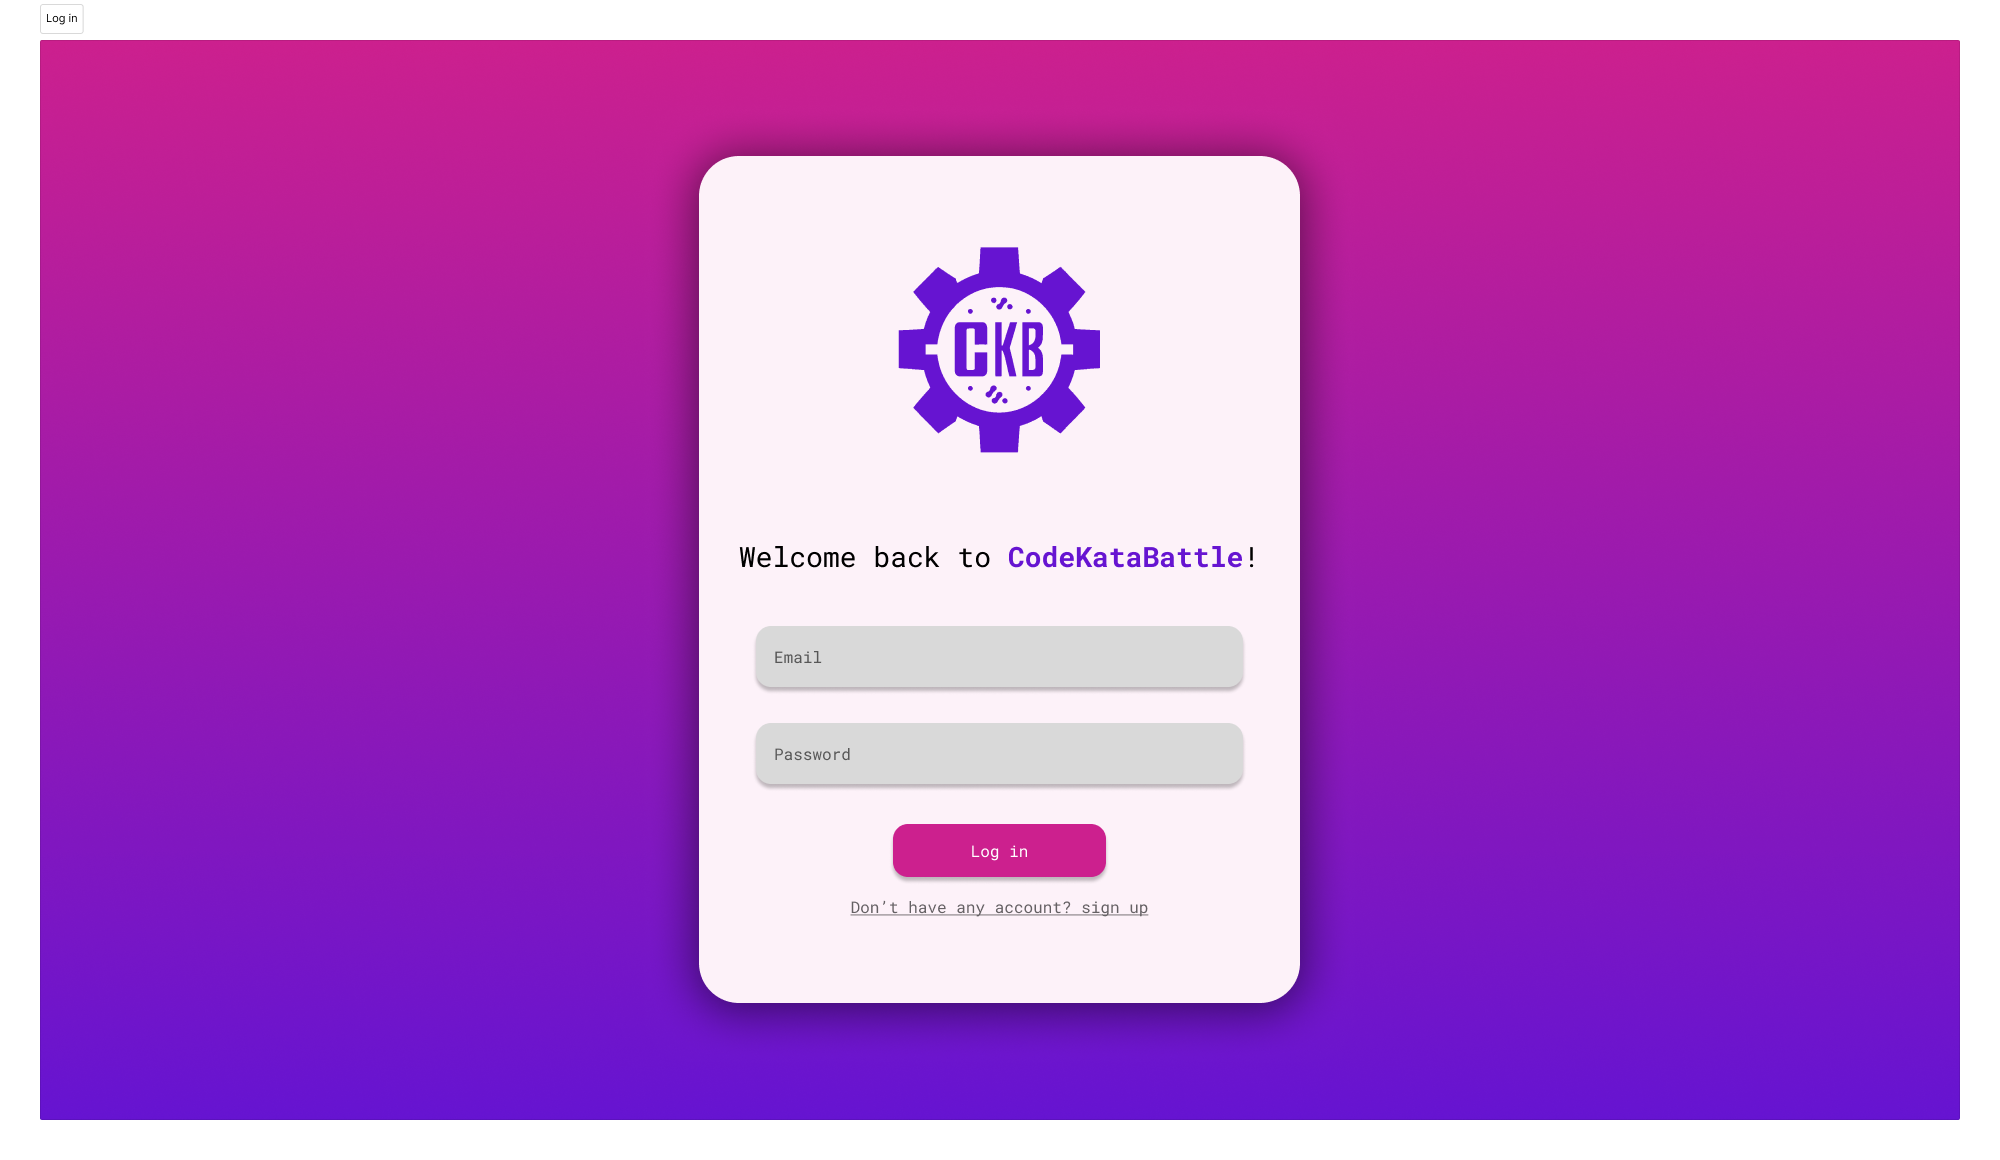
\includegraphics[width=1\textwidth]{images/user_interfaces/log_in.png}
    \caption{Log in page}
\end{figure}
\begin{figure}[H]
    \centering
    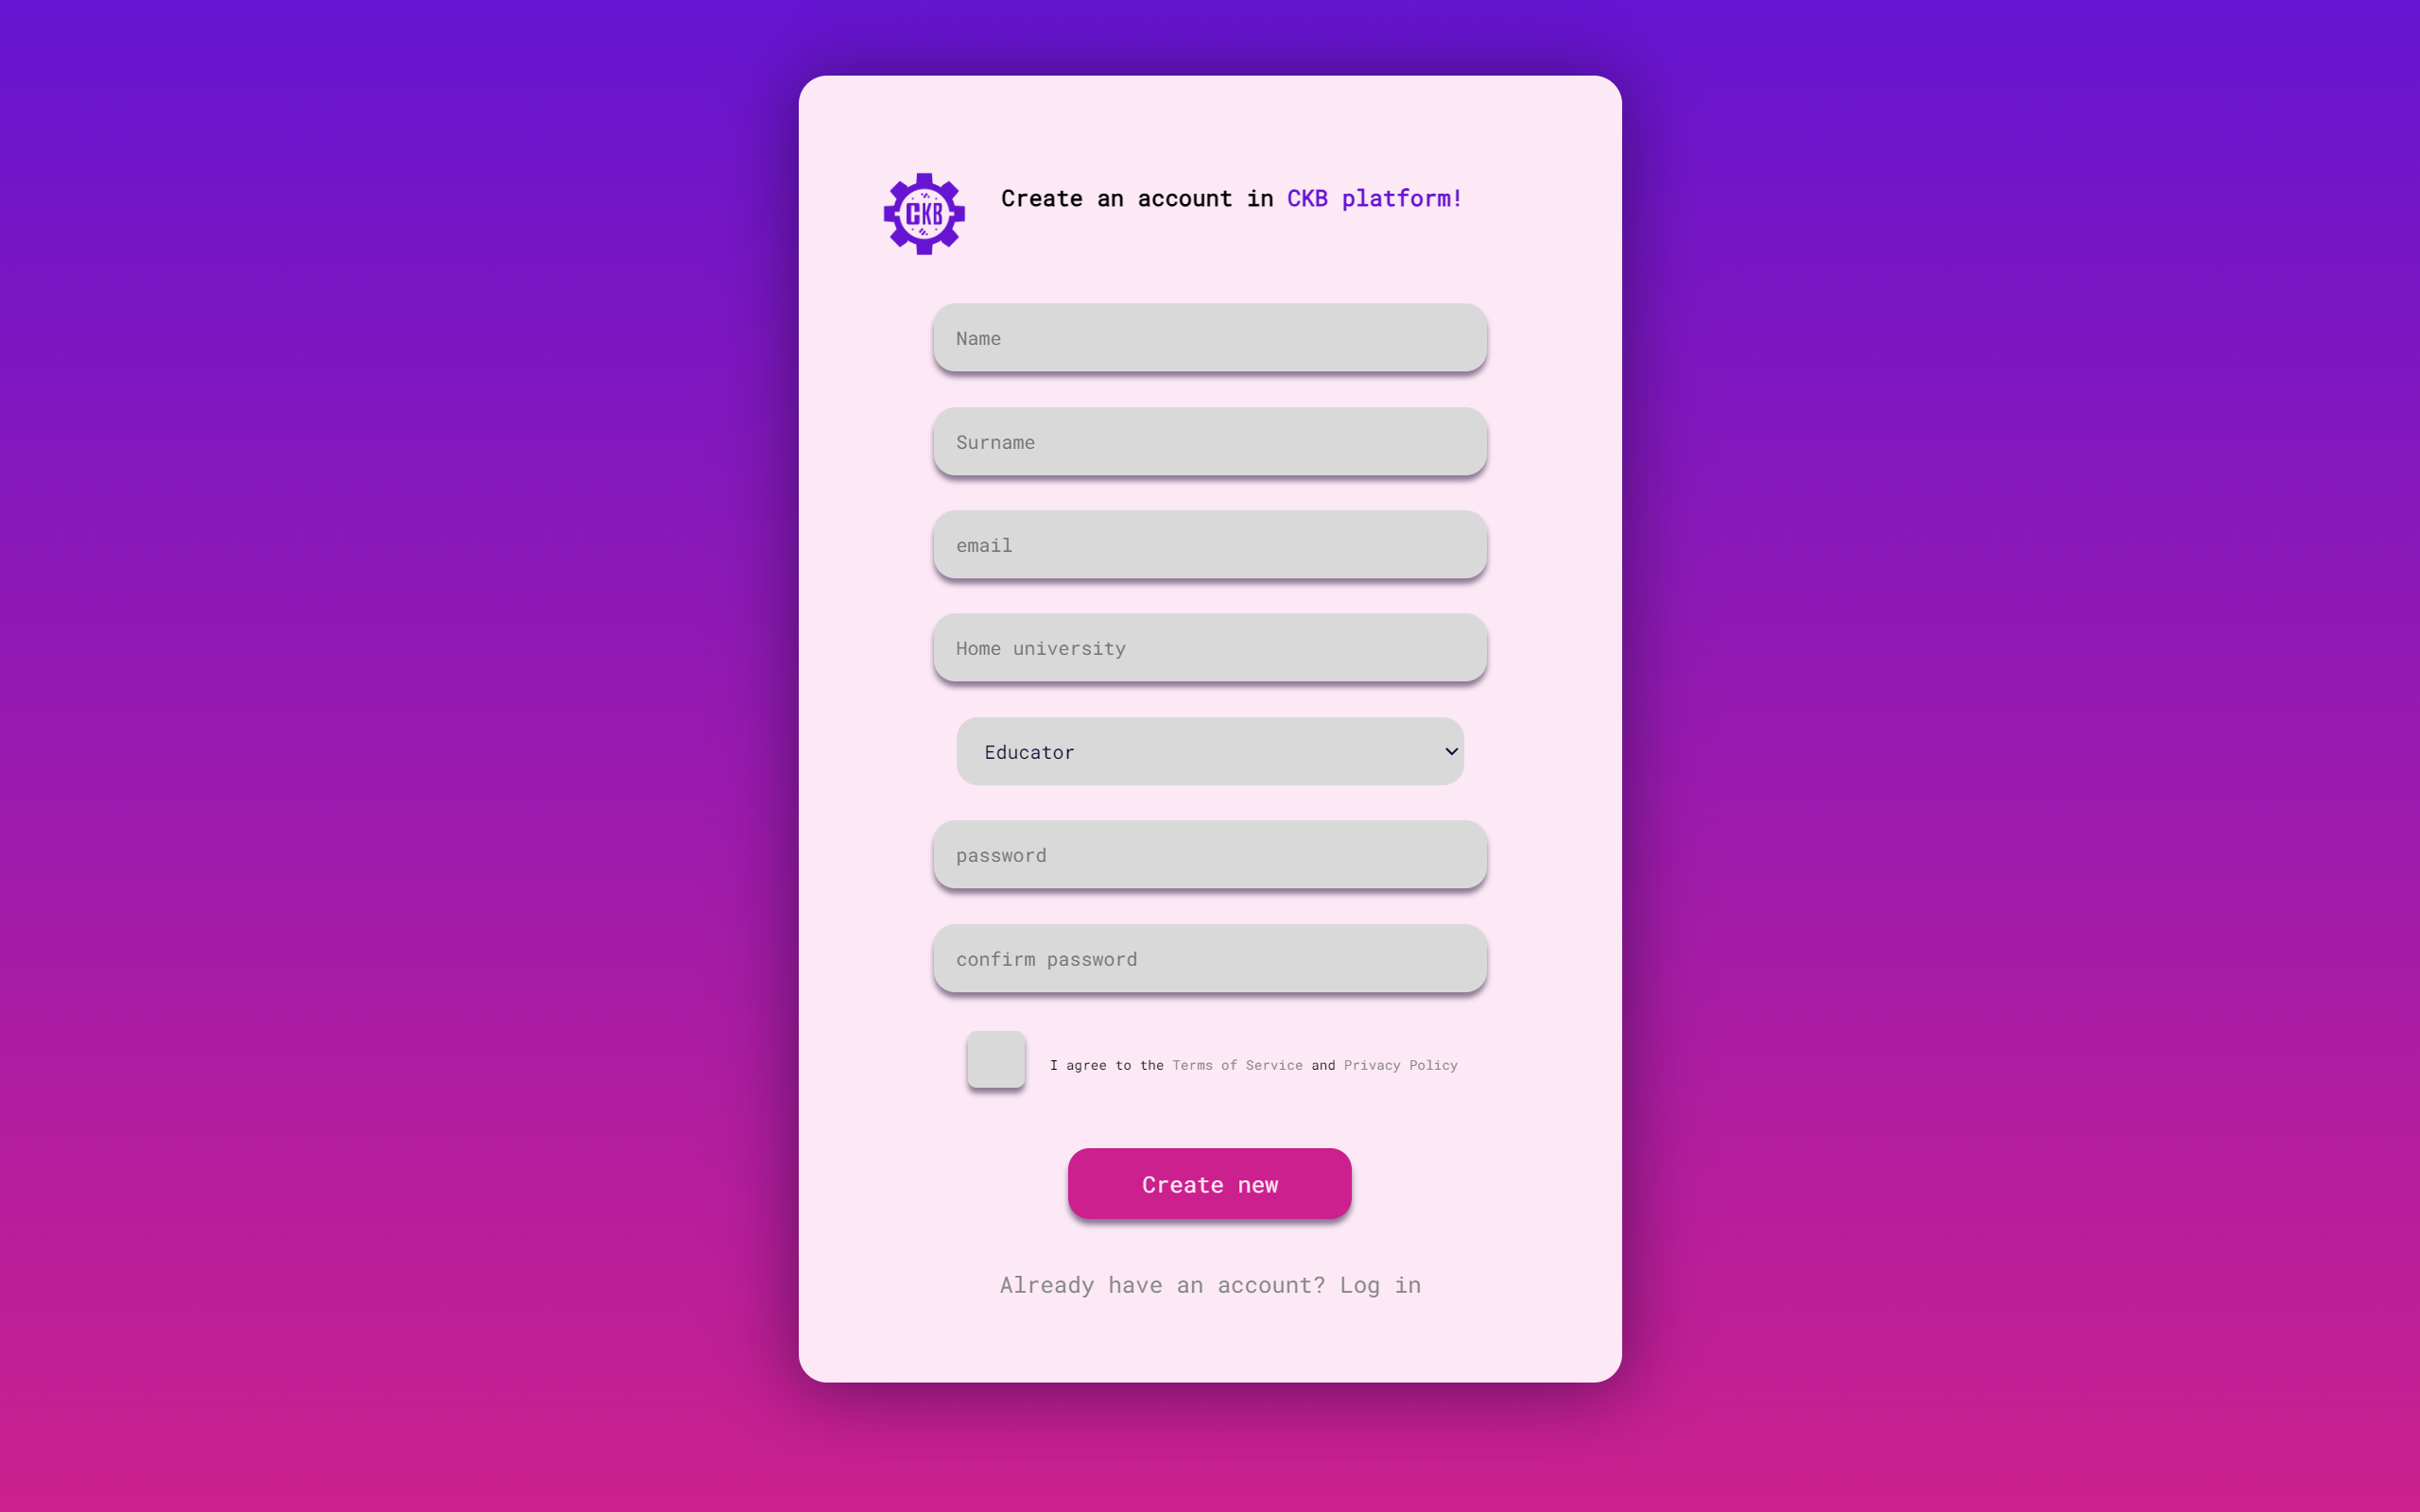
\includegraphics[width=1\textwidth]{images/user_interfaces/sign_up.png}
    \caption{Sign up page}
\end{figure}
\begin{figure}[H]
    \centering
    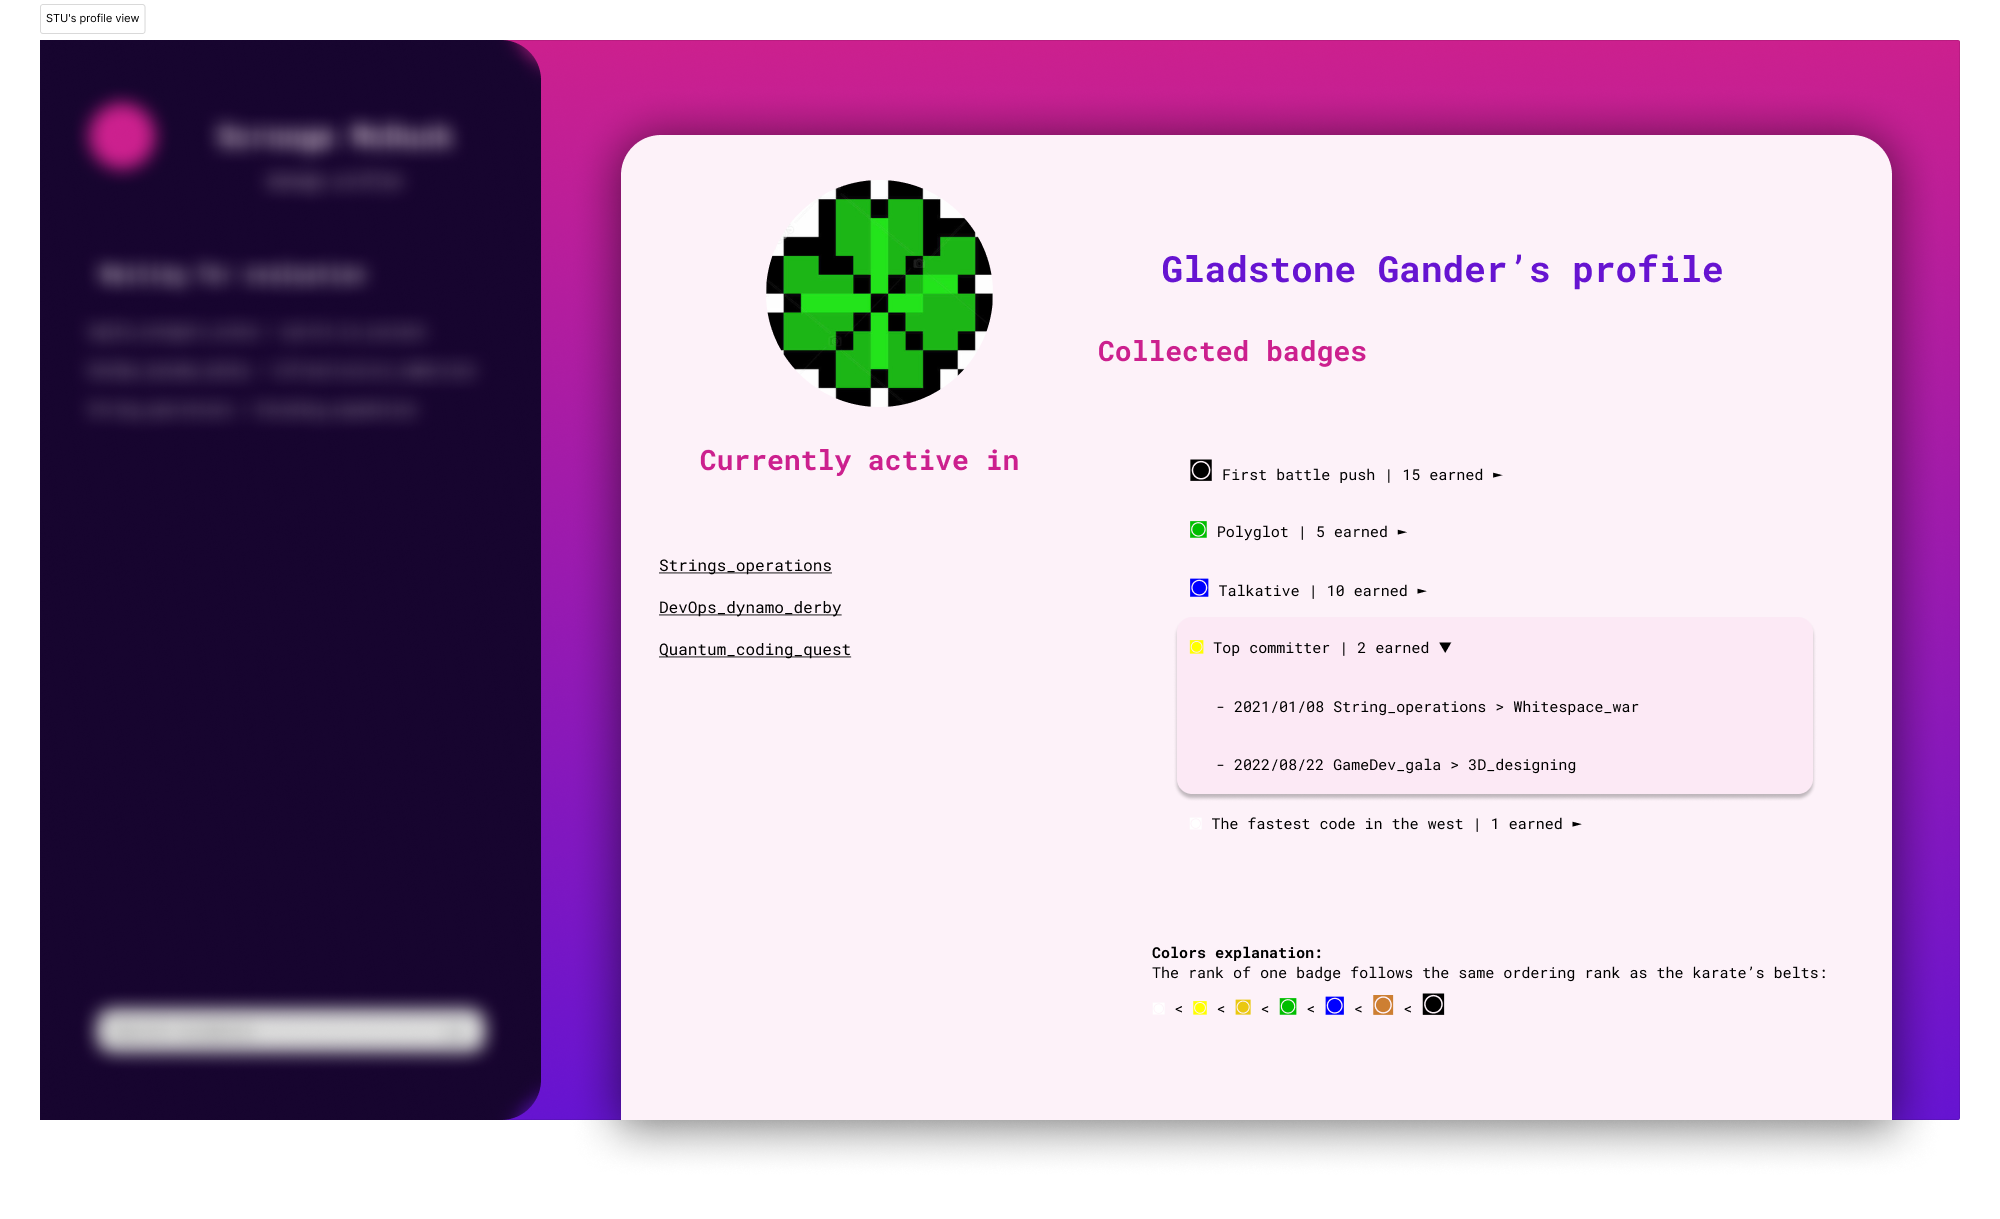
\includegraphics[width=1\textwidth]{images/user_interfaces/profile.png}
    \caption{Page that shows badges acquired by a STU}
\end{figure}

\subsubsection*{EDU's views}
\begin{figure}[H]
    \centering
    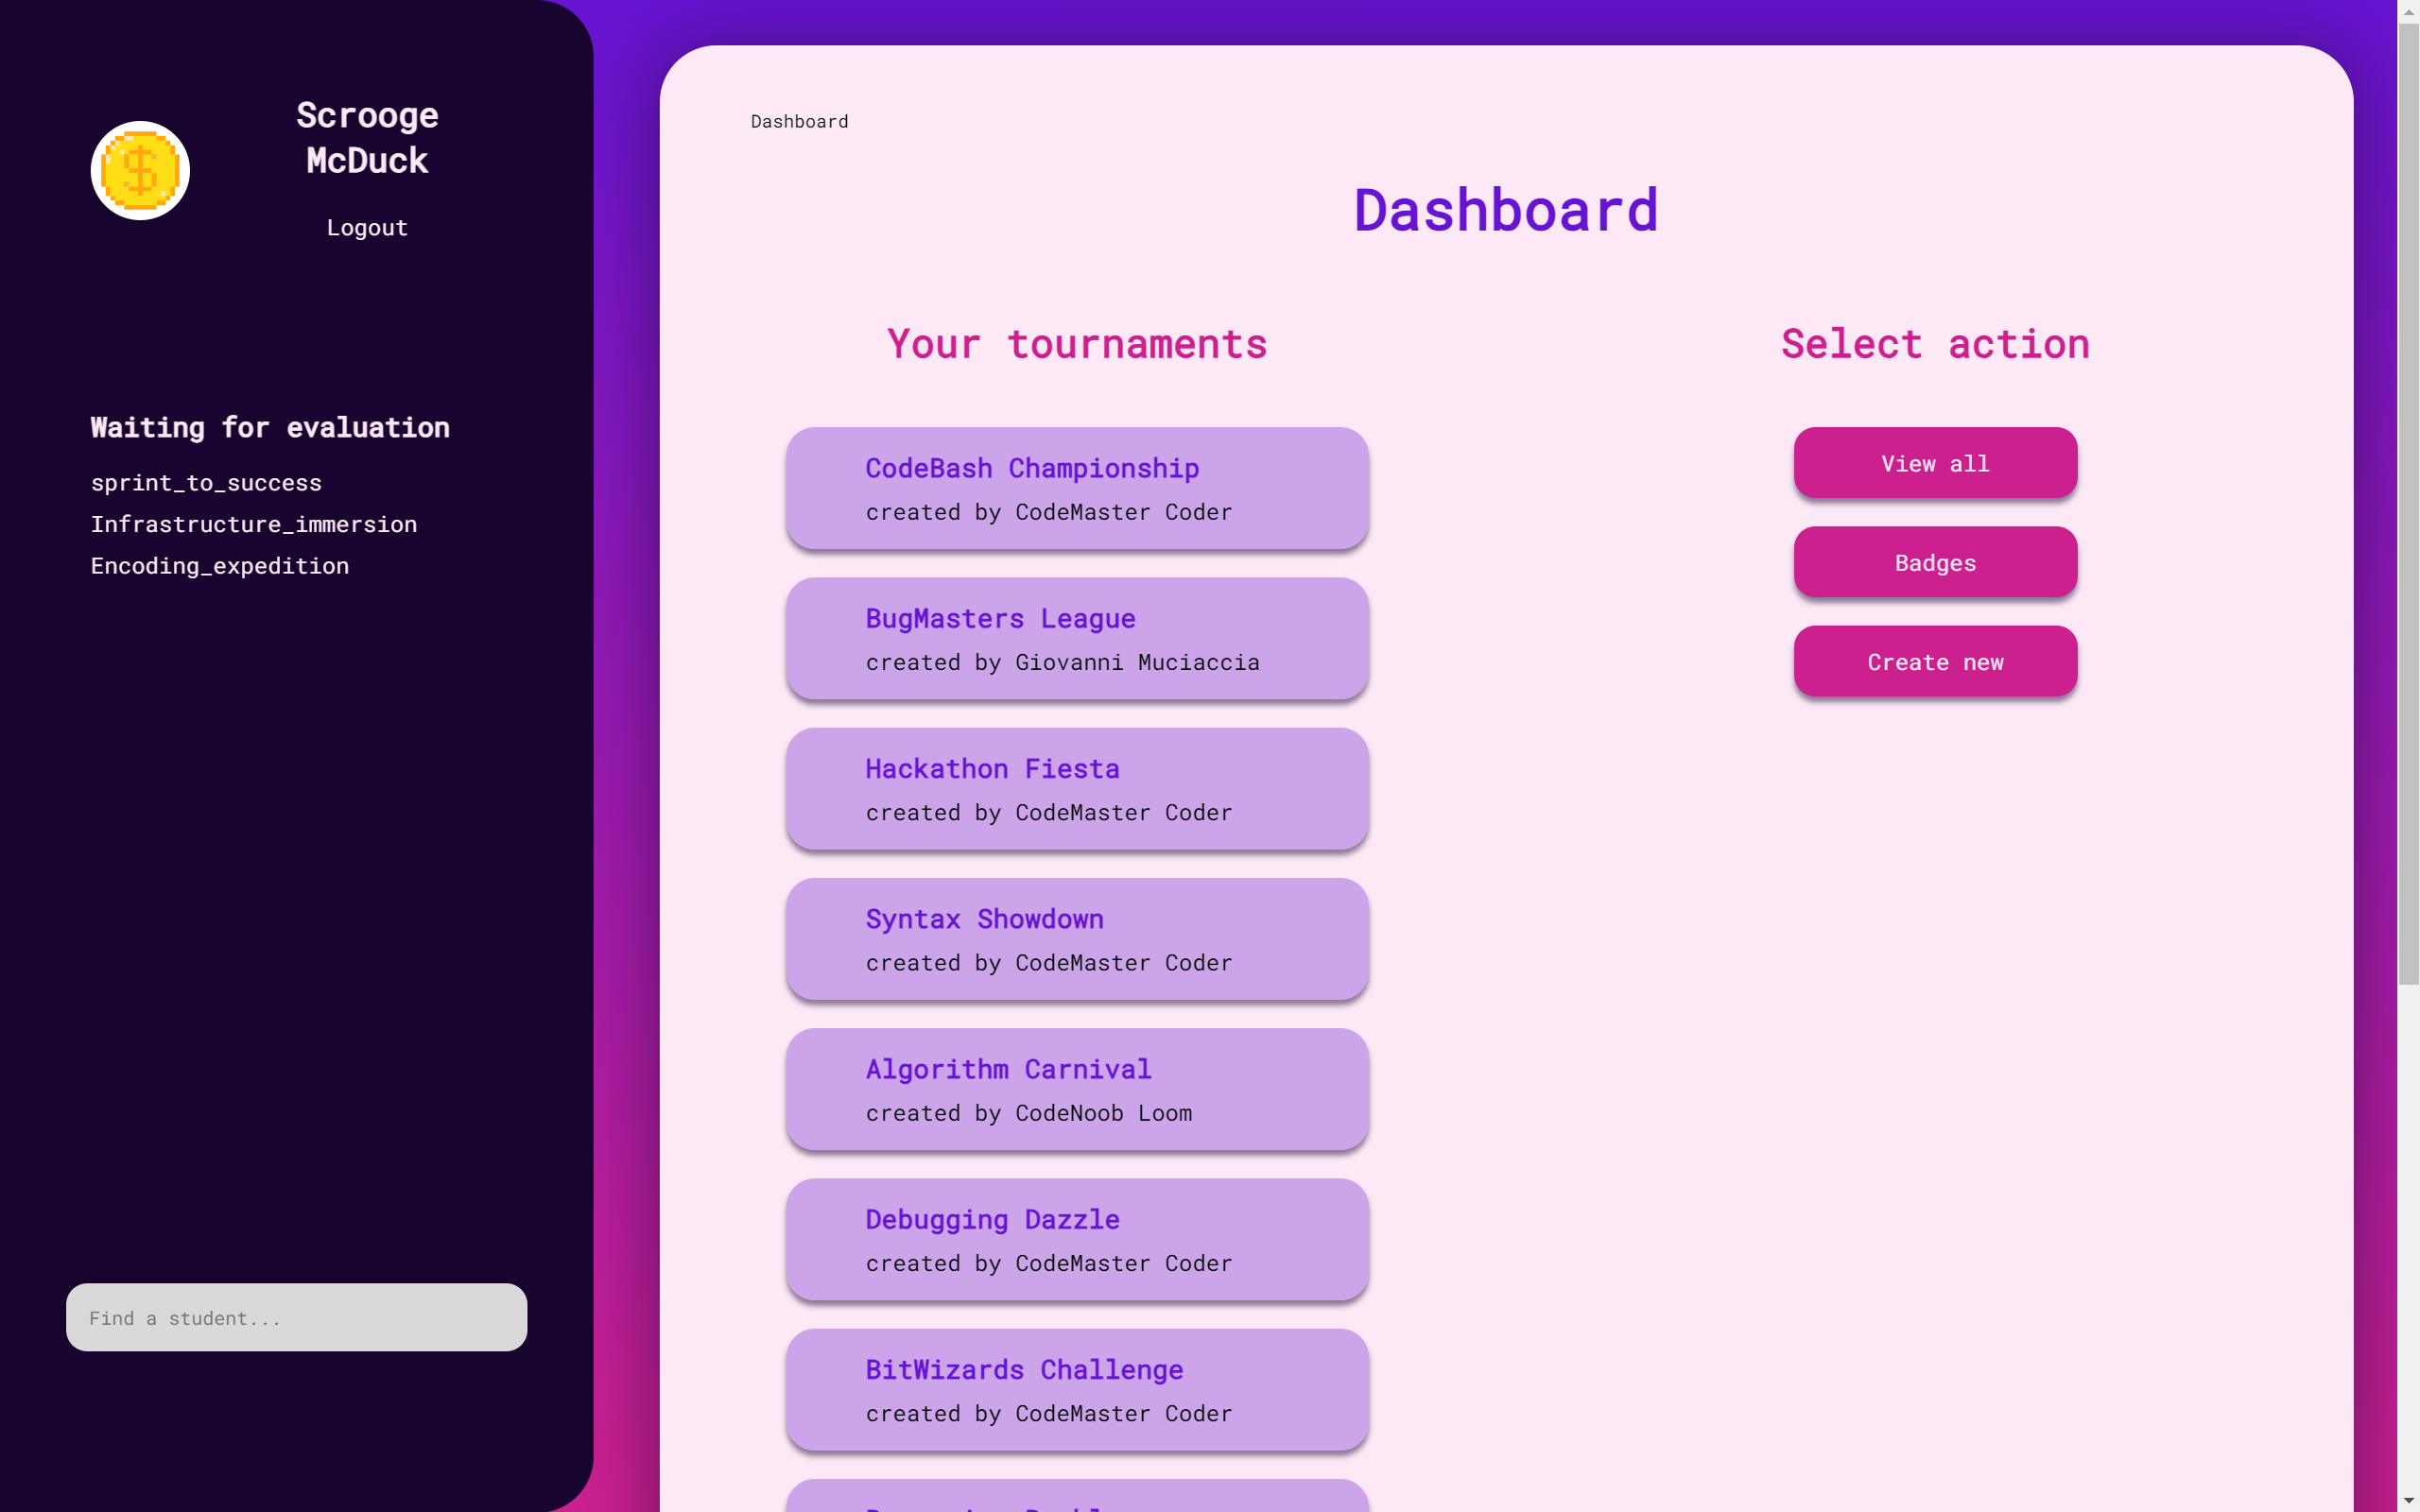
\includegraphics[width=1\textwidth]{images/user_interfaces/educator_dashboard.png}
    \caption{Dashboard}
\end{figure}
\begin{figure}[H]
    \centering
    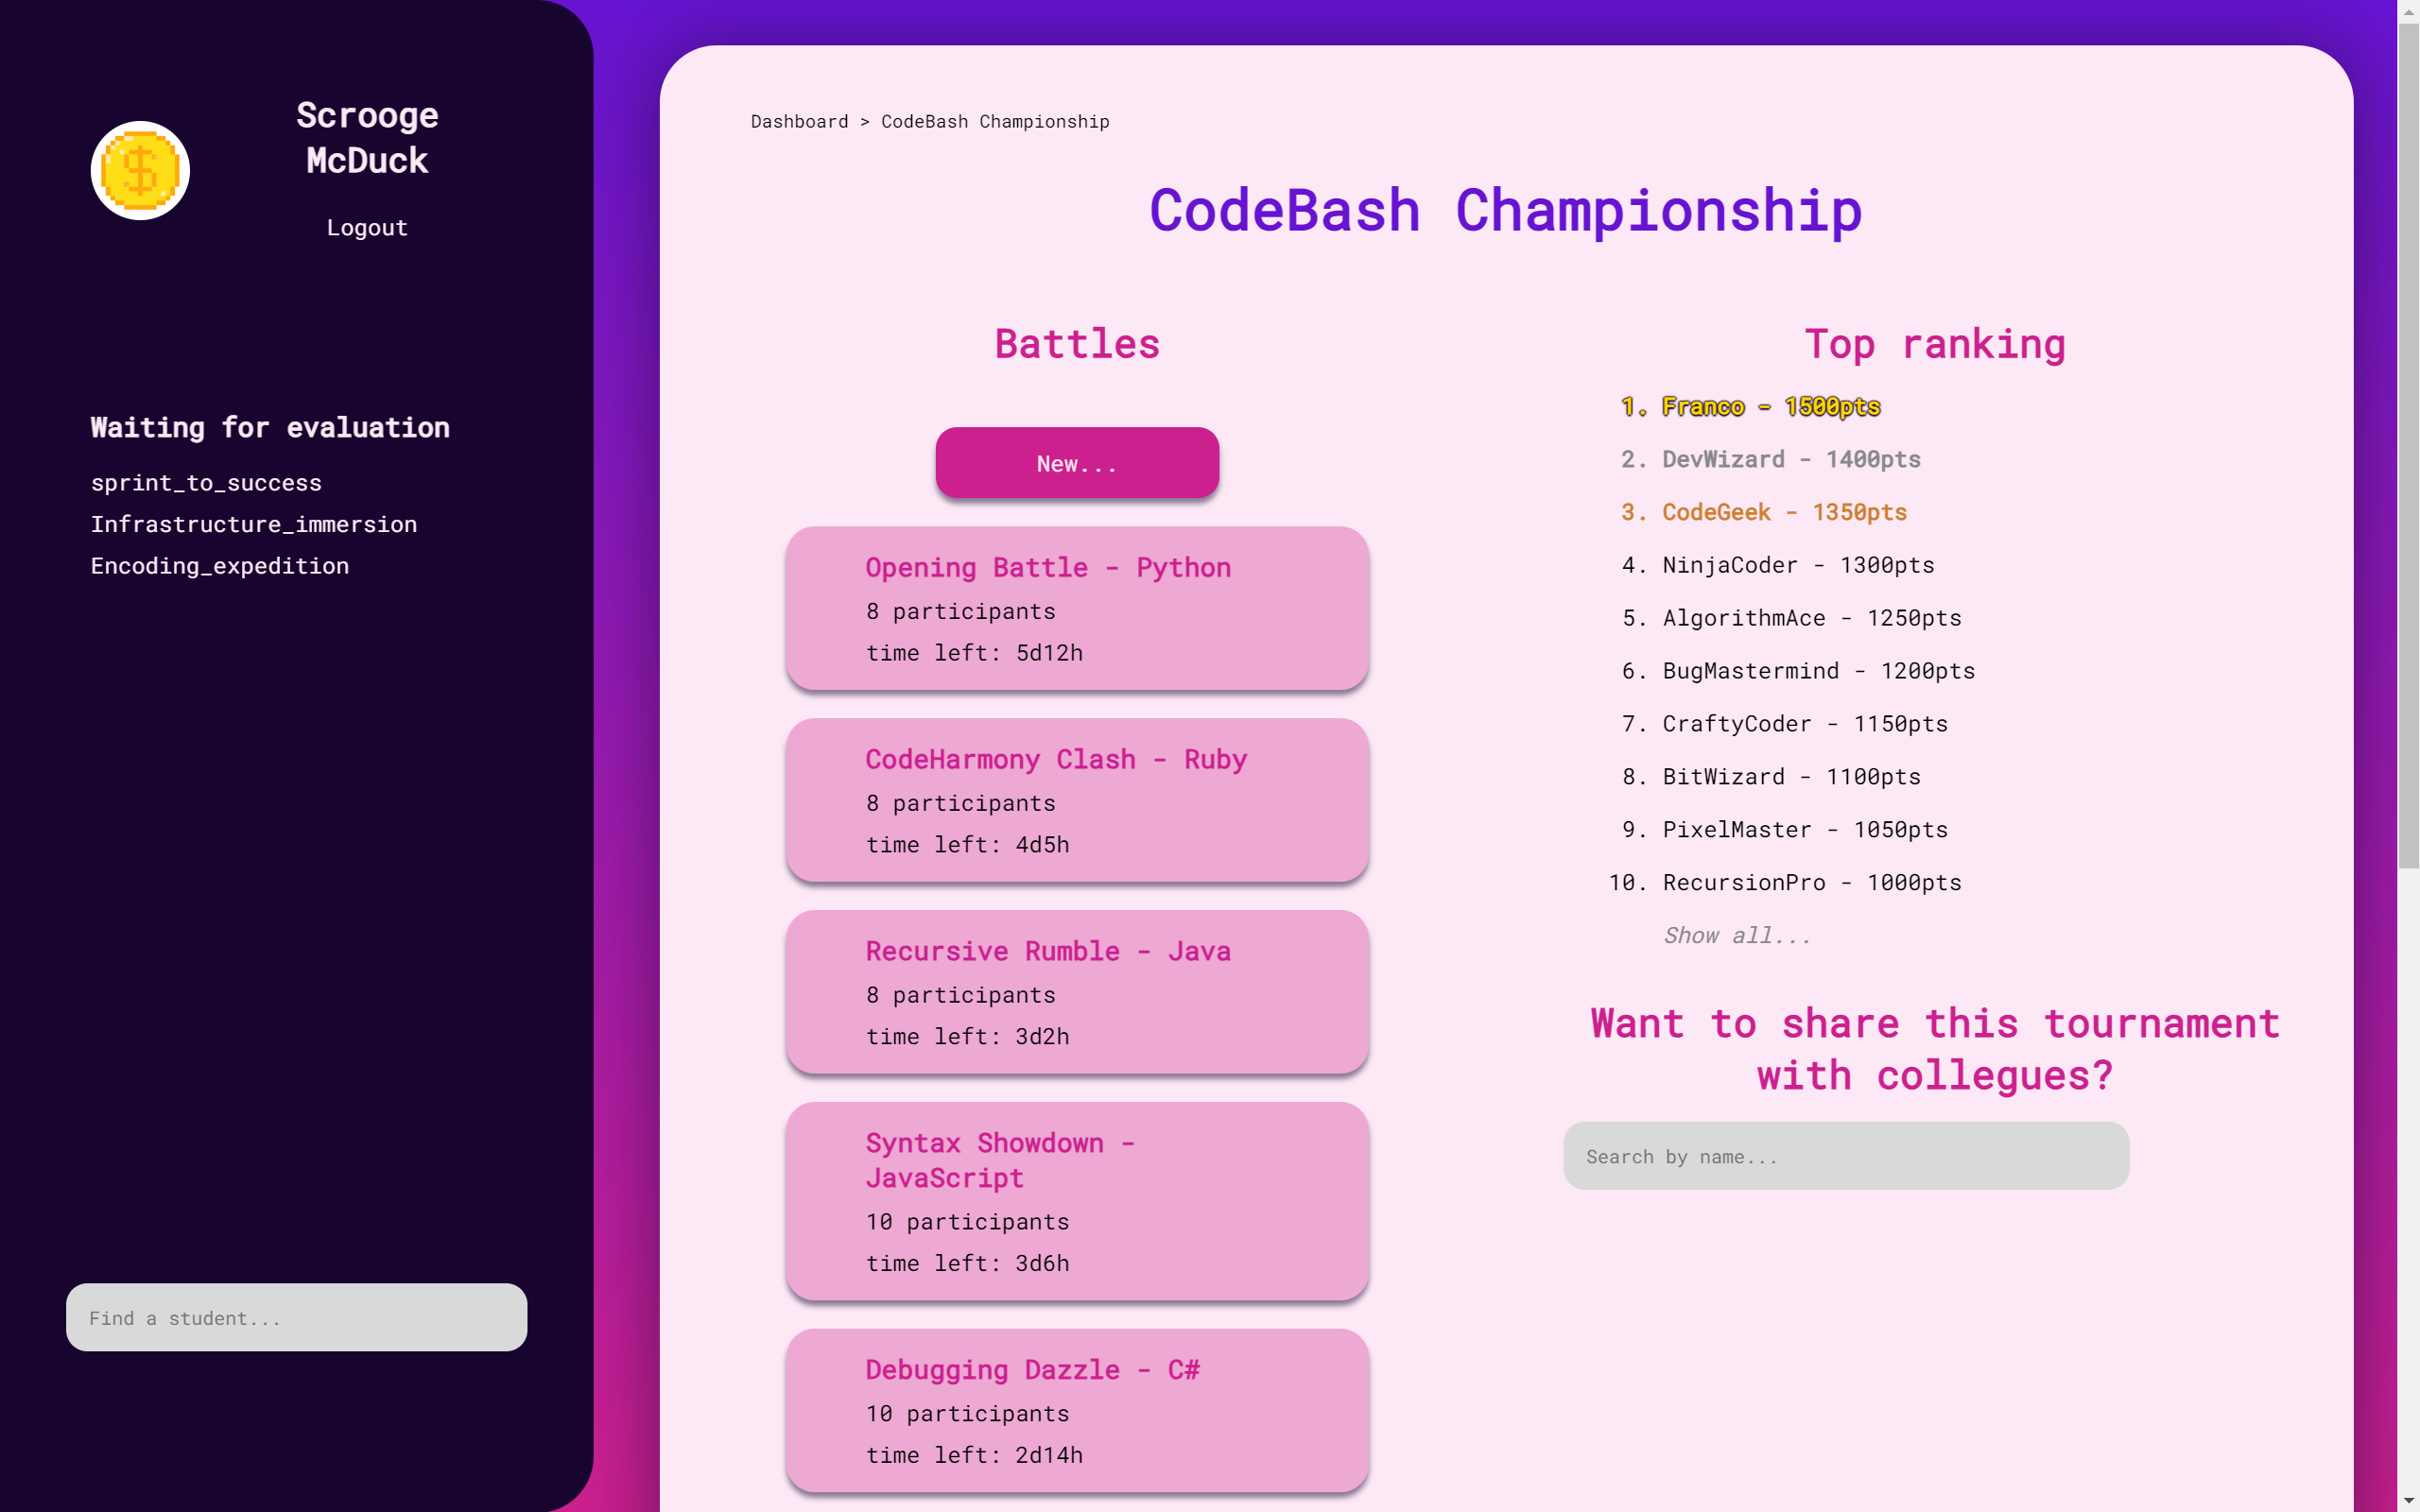
\includegraphics[width=1\textwidth]{images/user_interfaces/educator_tournament_view.png}
    \caption{View of a tournament}
\end{figure}
\begin{figure}[H]
    \centering
    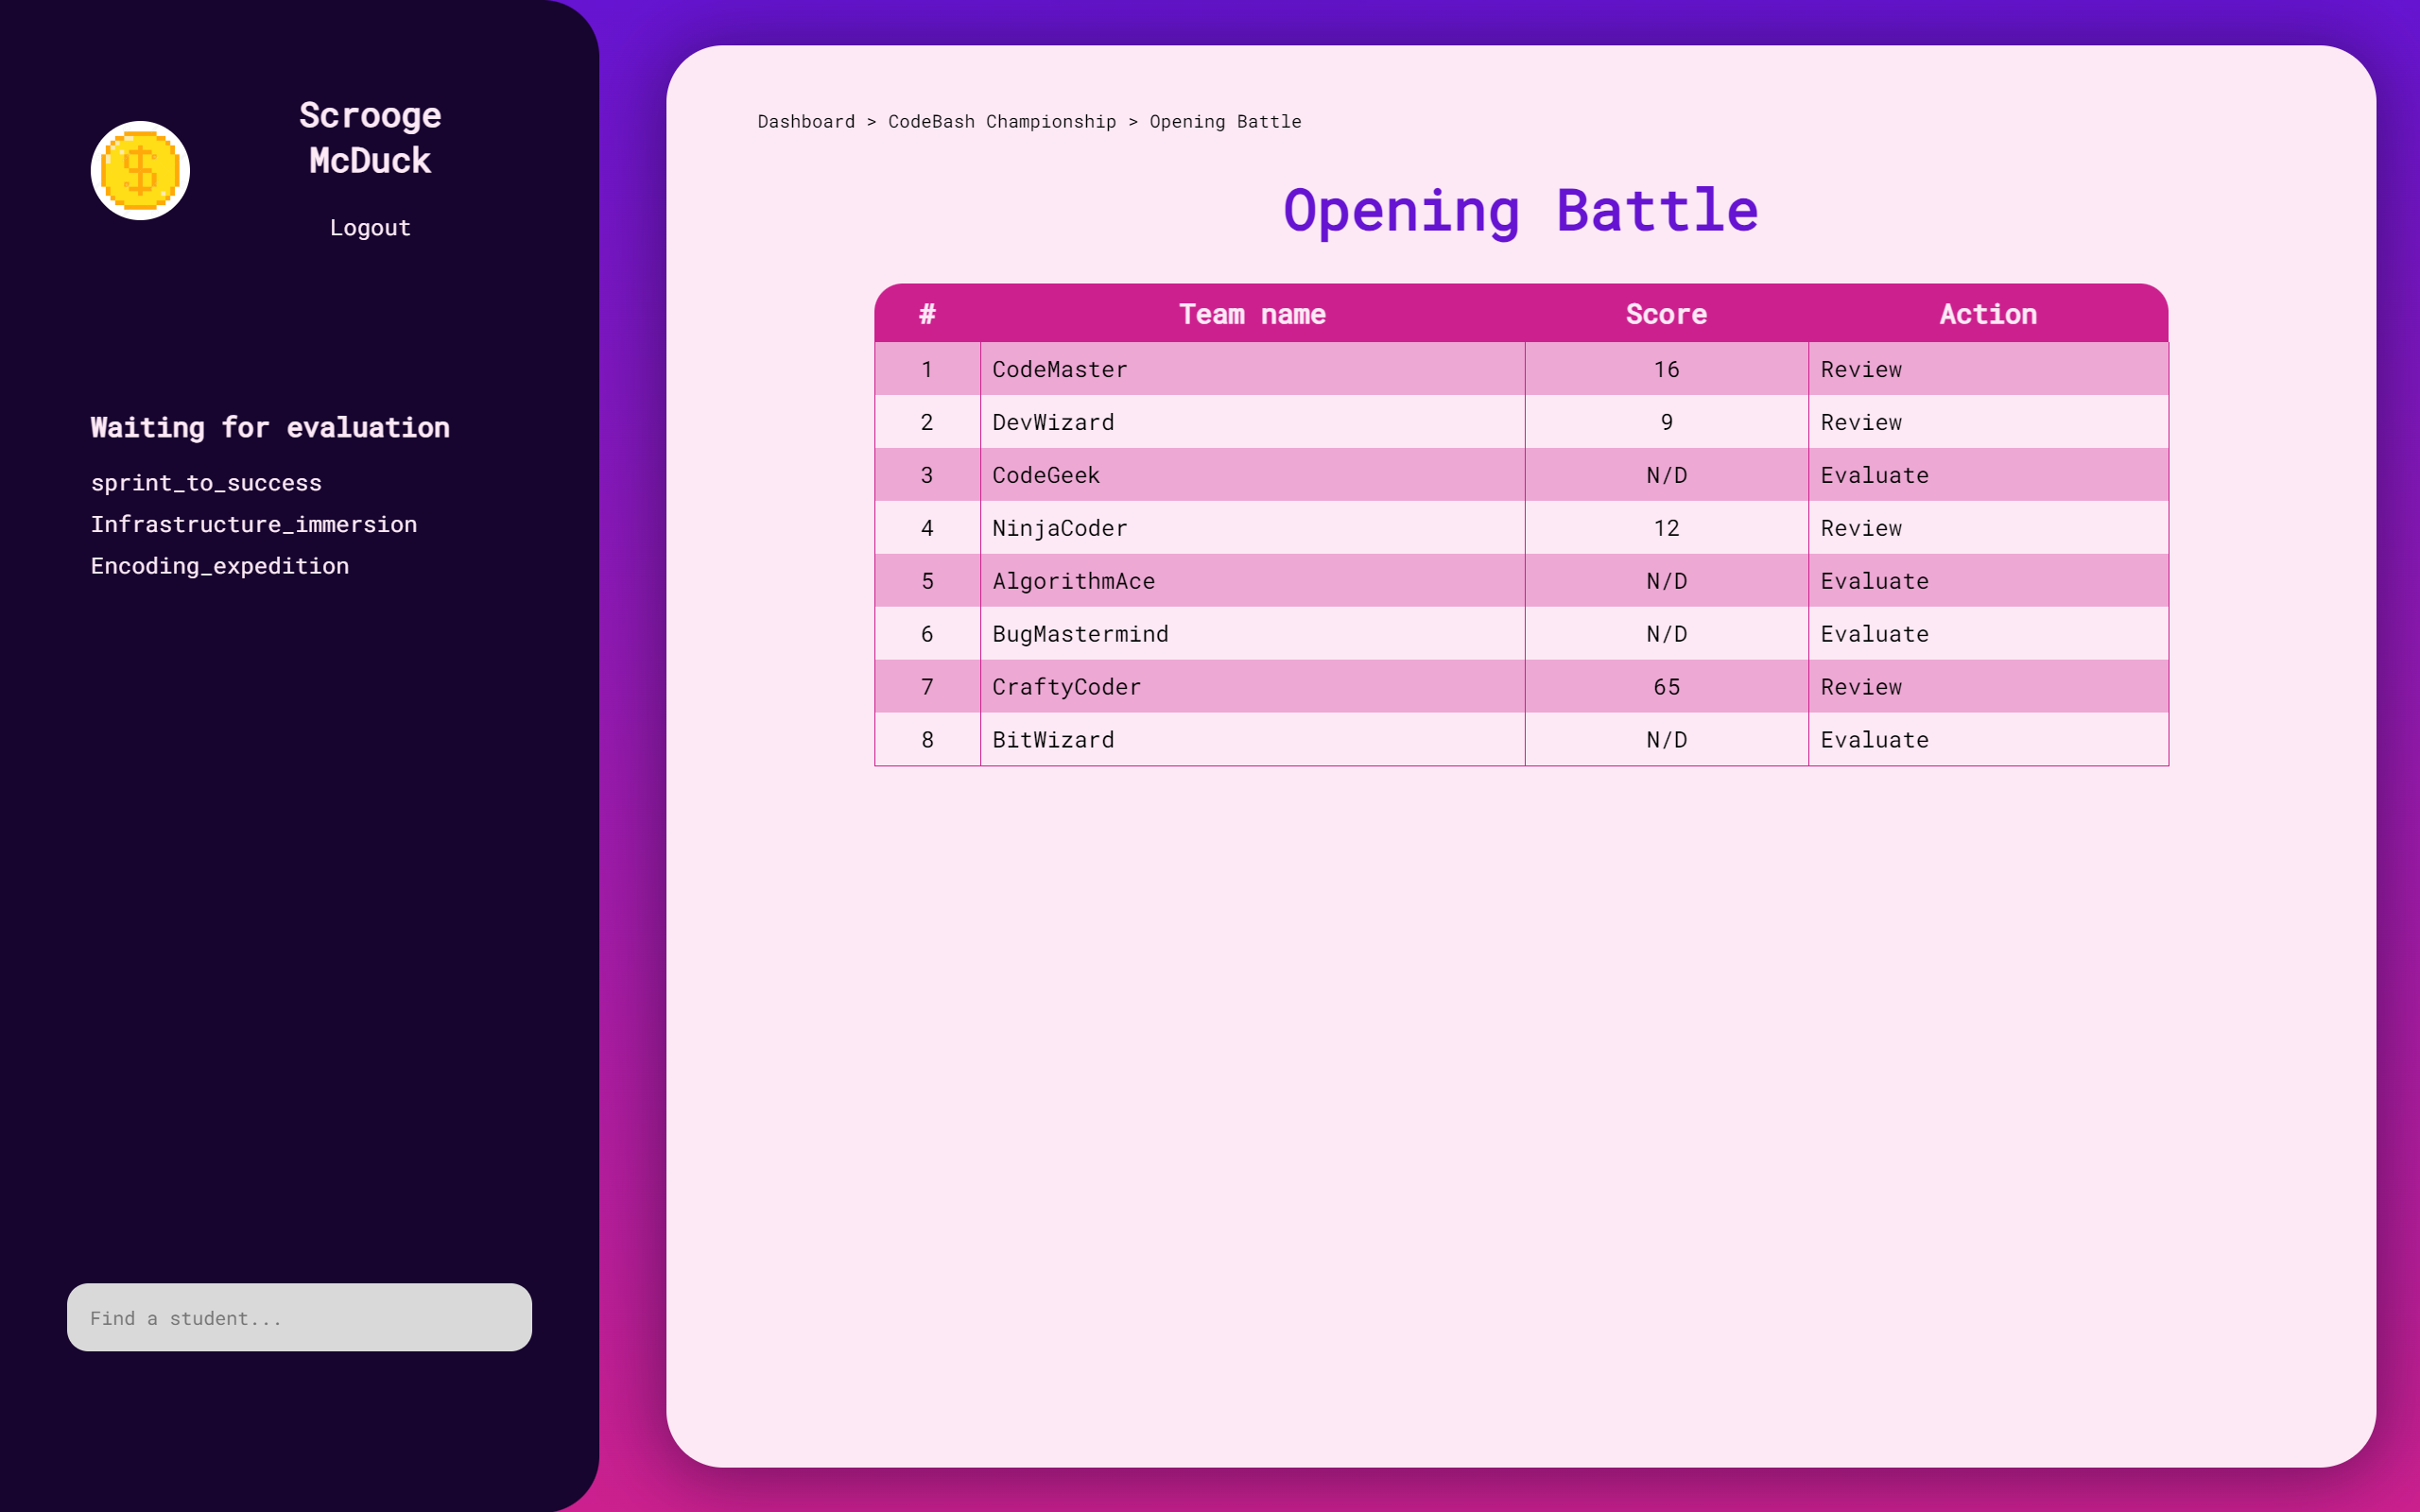
\includegraphics[width=1\textwidth]{images/user_interfaces/manual_evaluation.png}
    \caption{Manual evaluation page}
\end{figure}
\begin{figure}[H]
    \centering
    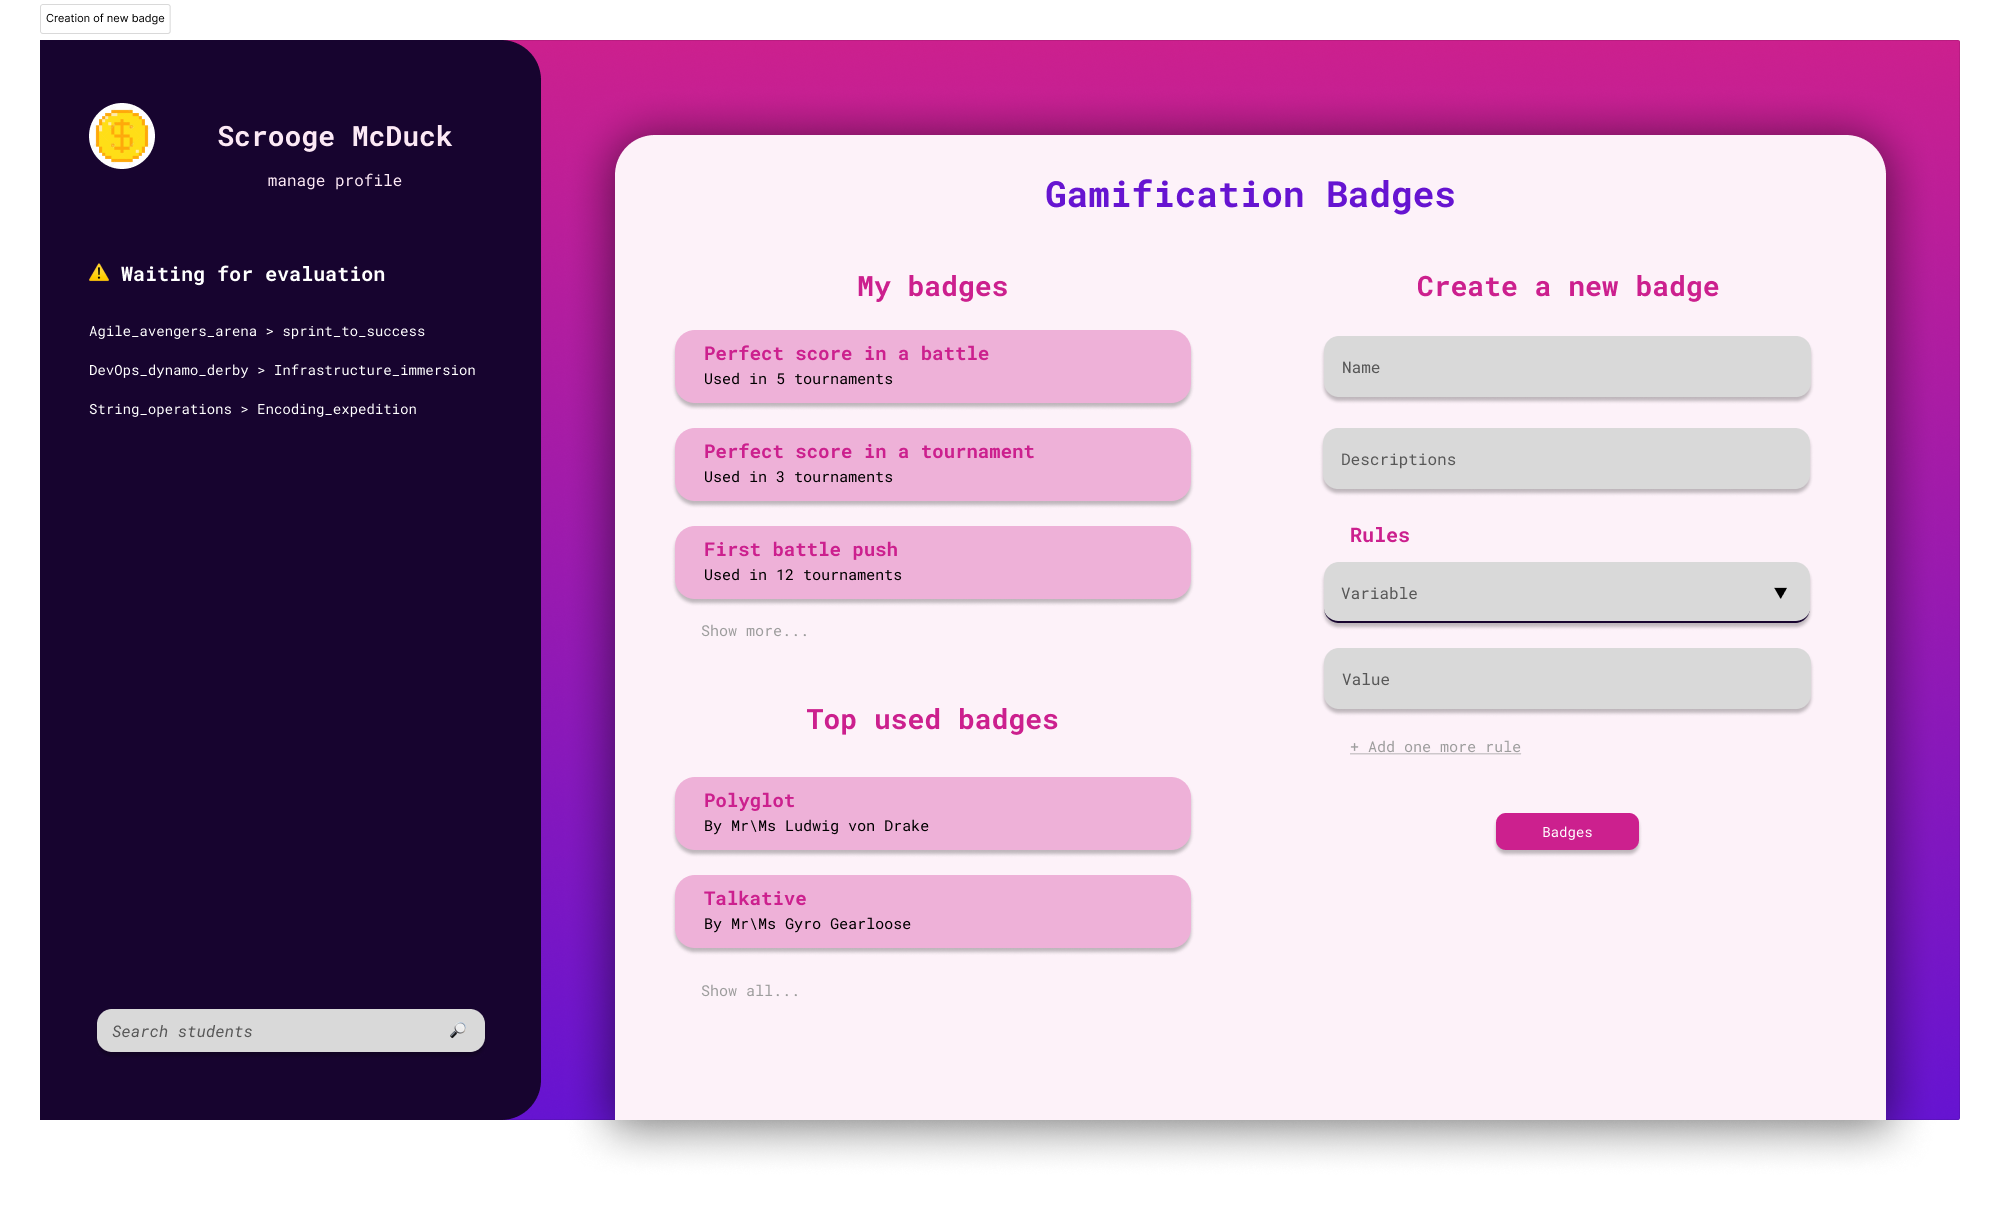
\includegraphics[width=1\textwidth]{images/user_interfaces/new_badge.png}
    \caption{Page to create a new badge}
\end{figure}

\subsubsection*{STU's views}
\begin{figure}[H]
    \centering
    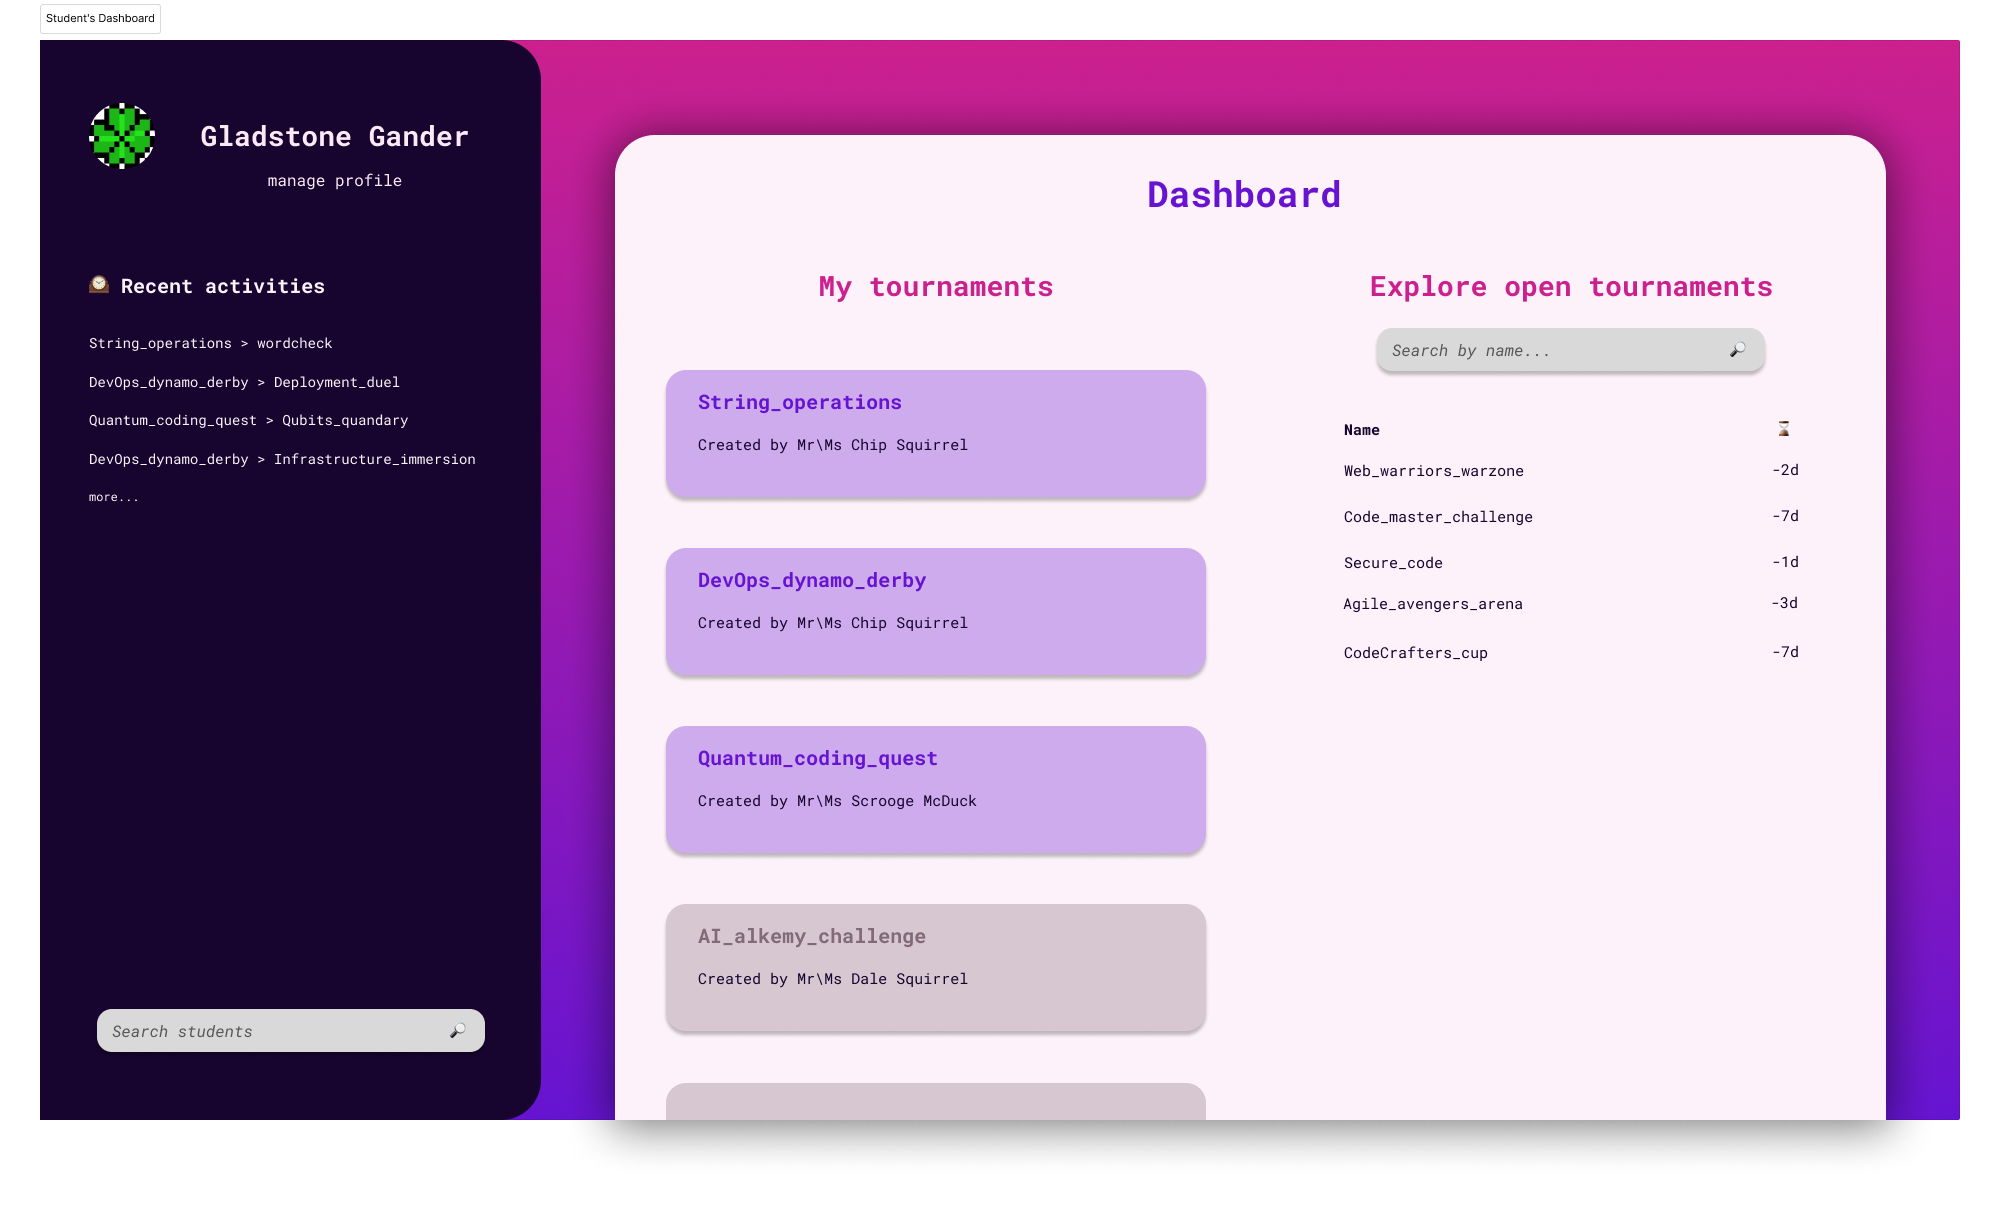
\includegraphics[width=1\textwidth]{images/user_interfaces/student_dashboard.png}
    \caption{Dashboard}
\end{figure}
\begin{figure}[H]
    \centering
    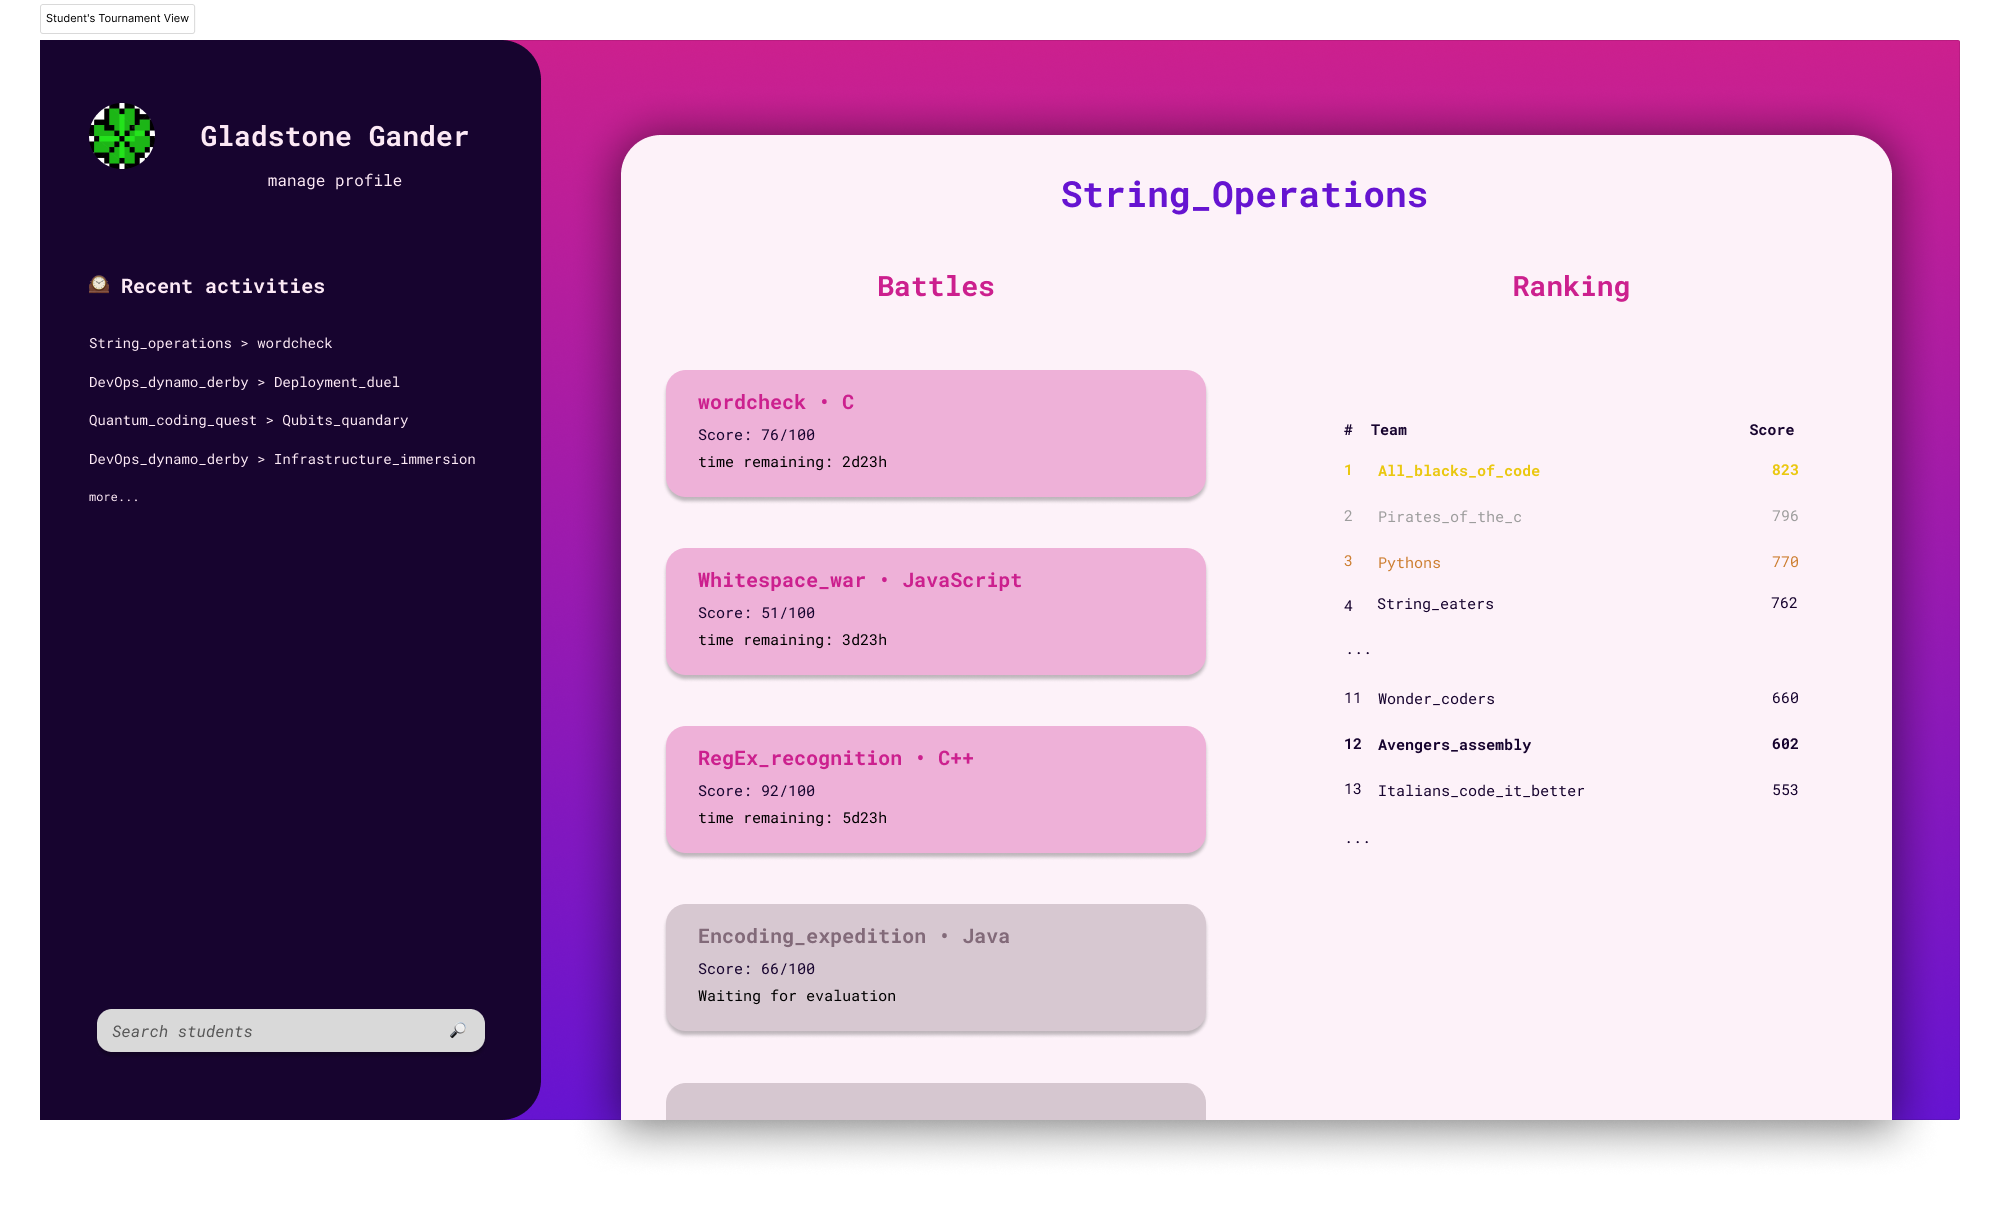
\includegraphics[width=1\textwidth]{images/user_interfaces/student_tournament_view.png}
    \caption{View of a tournament}
\end{figure}
\begin{figure}[H]
    \centering
    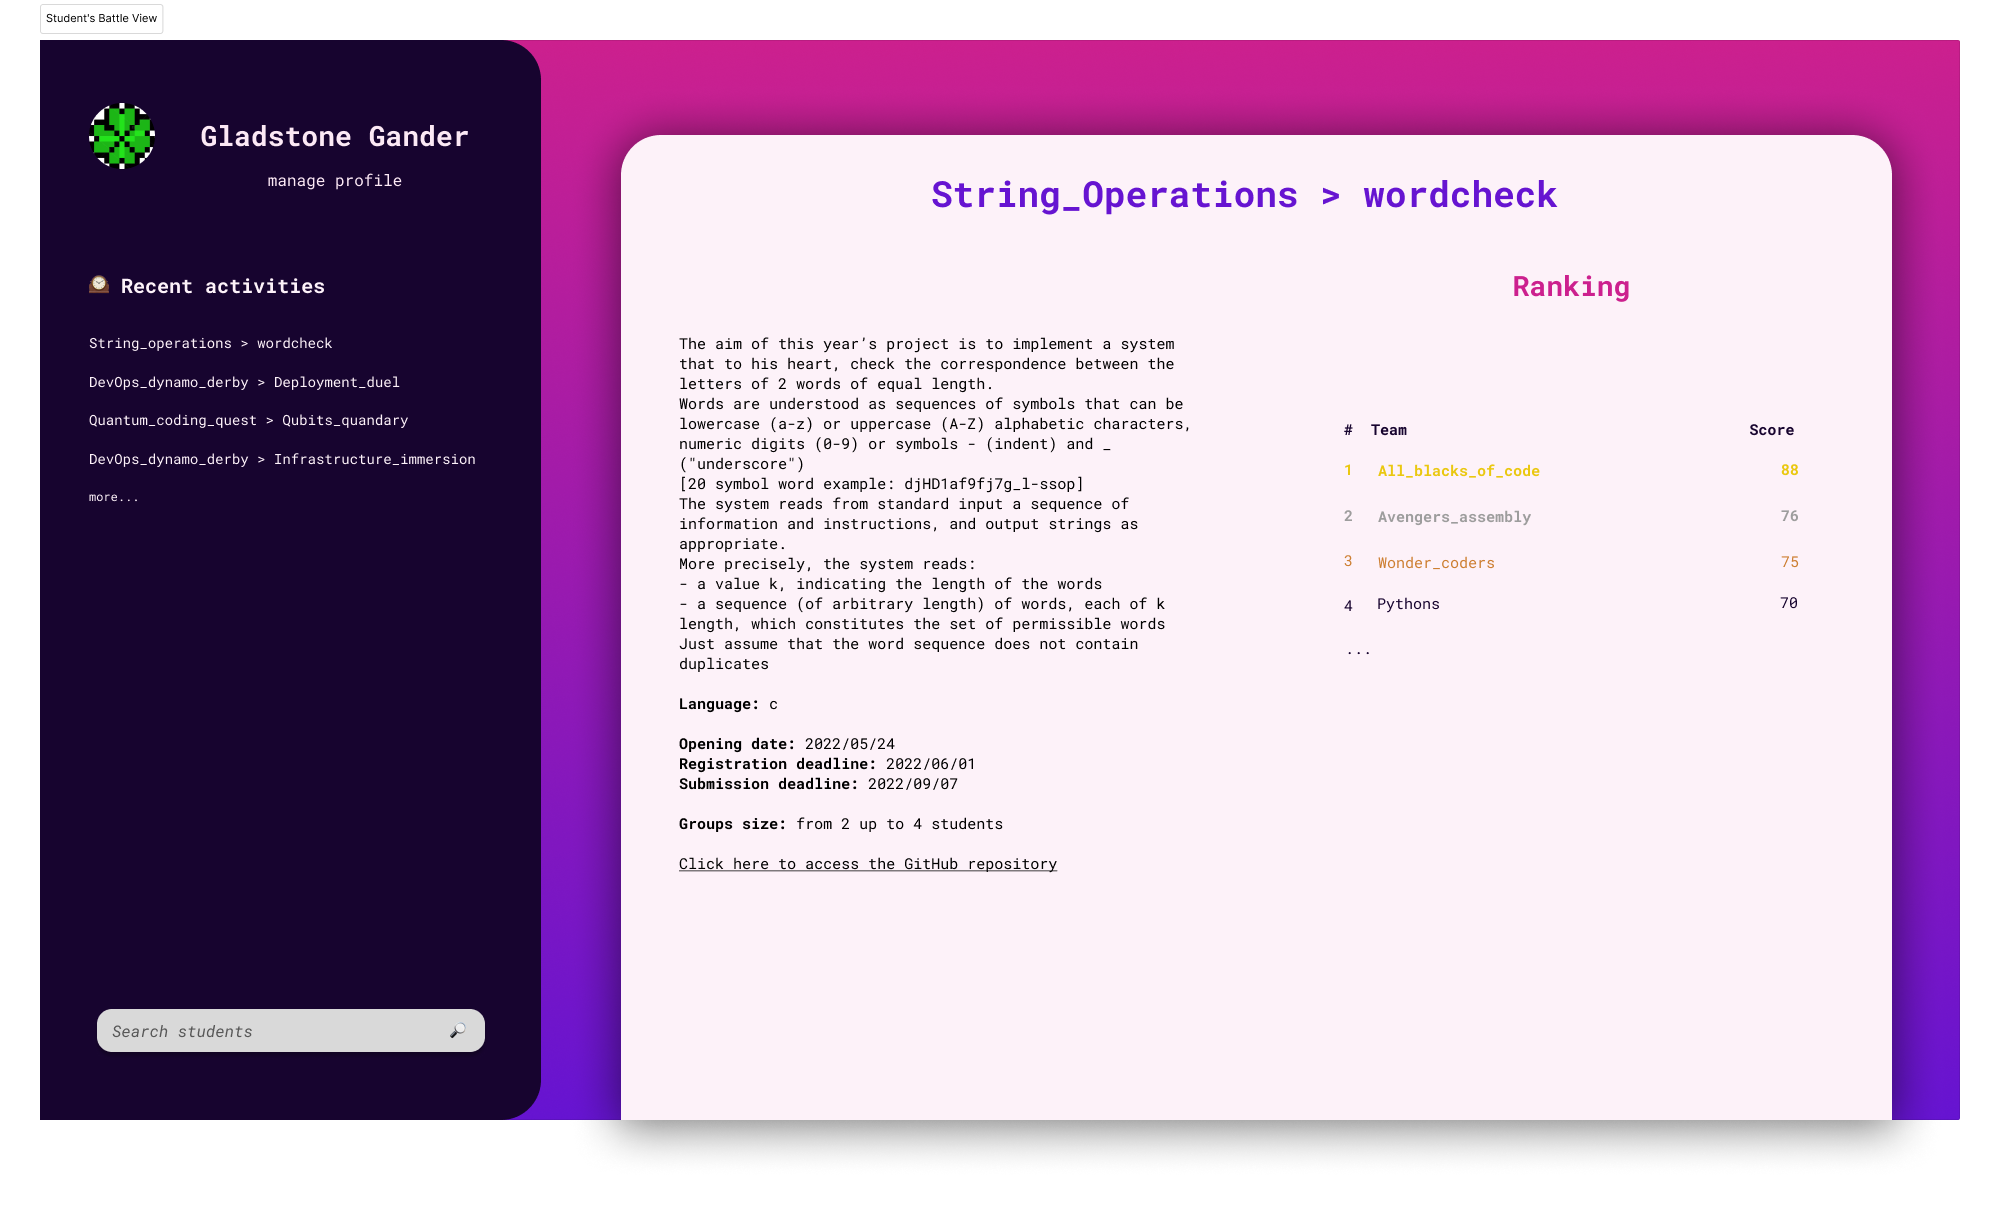
\includegraphics[width=1\textwidth]{images/user_interfaces/student_battle_view.png}
    \caption{View of a battle}
\end{figure}



\subsection{Hardware Interfaces}
To use the CKB platform, both the Educators and the Students need an electronic device connected to the Internet, like a computer, a tablet or a smartphone.\\
As the platform's primary functionality is closely tied to coding activities, it is expected that users will predominantly employ personal computers to access an Integrated Development Environment (IDE). Consequently, the platform's interfaces have been optimized for use on computer screens.

\subsection{Software Interfaces}
Since the platform is web-based, it is compatible with all the major operating systems, as long as they have a modern browser installed.

\subsection{Communication Interfaces}
The system requires a stable internet connection to work properly. The backend of the system will expose a unified RESTful API to communicate with all clients.\\
Furthermore, he system relies on various external interfaces accessible via uniform web API. These services are:
\begin{itemize}
    \item \textbf{GitHub API:} to create and manage repositories and to retrieve the code of the students and to authenticate users.
    \item \textbf{Mail API:} to send emails to the users to notify them about events.
\end{itemize}

\section{Functional Requirements}
In order to work properly, the software must fulfill the following functional requirements, which are written in hierarchical order, starting from the requirements of EDUs agents and then STUs agents\dots

\subsection{Use cases Diagrams}

\subsection{Use cases Description}

%% LAYOUT FOR THE TABLES:
% \begin{center}
%     \def\arraystretch{1.5}
%     \setlist[enumerate]{itemsep=.1pt}
%     \begin{tabular}{| m{2cm} | m{10cm}|}
%         \hline
%         Name                  &  \\ \hline
%         ID                    &  \\ \hline
%         Actors                &  \\ \hline
%         Entry \par conditions &  \\ \hline
%         Event \par flow            & \begin{enumerate}
%                                     \item
%                                     \item
%                                     \item
%                                     \item
%                                 \end{enumerate}                              \\ \hline
%         Exit \par conditions       &                                               \\ \hline
%         Exceptions            &                                               \\ \hline
%         Notes                &                                               \\ \hline   
%     \end{tabular}
% \end{center}

\begin{center}
    \def\arraystretch{1.5}
    \setlist[enumerate]{itemsep=.1pt}
    \begin{tabular}{| m{2cm} | m{10cm}|}
        \hline
        Name                  & Register                                                                                  \\ \hline
        ID                    & UC1                                                                                       \\ \hline
        Actors                & EDU or STU                                                                                \\ \hline
        Entry \par conditions & The actor is not registered and wants to create an account                                \\ \hline
        Event \par flow       & \begin{enumerate}
                                    \item The actor enters the registration page
                                    \item The system shows the registration form
                                    \item The actor decides whether he is an educator or a student
                                    \item The actor fills the form with truthful informations
                                    \item The actor confirm the account creation
                                    \item The system creates an account with respect to the informations inserted by the actor
                                \end{enumerate} \\ \hline
        Exit \par conditions  & The system creates successfully the account                                               \\ \hline
        Exceptions            & The actor inserts informations (i.e. email) about an account which already exists         \\ \hline
    \end{tabular}
\end{center}

\begin{center}
    \def\arraystretch{1.5}
    \setlist[enumerate]{itemsep=.1pt}
    \begin{tabular}{| m{2cm} | m{10cm}|}
        \hline
        Name                  & Log in                                                                                              \\ \hline
        ID                    & UC2                                                                                                 \\ \hline
        Actors                & EDU or STU                                                                                          \\ \hline
        Entry \par conditions & The actor is already subscribed to the CKB platform                                                 \\ \hline
        Event \par flow       & \begin{enumerate}
                                    \item The actor enters the login page
                                    \item The system shows the login form
                                    \item The actor fills the form with its credentials and submits it
                                    \item The system checks the credentials and logs the actor in
                                \end{enumerate}                                   \\ \hline
        Exit \par conditions  & The actor is logged in and it has access to the home page                                           \\ \hline
        Exceptions            & The actor inserts a wrong combination of username - password: a human-readable message is displayed \\ \hline
    \end{tabular}
\end{center}
\begin{center}
    \def\arraystretch{1.5}
    \setlist[enumerate]{itemsep=.1pt}
    \begin{tabular}{| m{2cm} | m{10cm}|}
        \hline
        Name                  & Battle creation                                                                                          \\ \hline
        ID                    & UC4                                                                                                      \\ \hline
        Actors                & EDU                                                                                                      \\ \hline
        Entry \par conditions & The actor is already subscribed to the CKB platform and he is an educator already logged in the platform \\ \hline
        Event \par flow       & \begin{enumerate}
                                    \item The actor opens the page correlated to the tournament in which he wants to create a new battle
                                    \item The system shows the tournament page
                                    \item If the actor has enough permissions, the system shows the "create a new battle" button
                                    \item The actor opens the battle creation page
                                    \item The system shows the battle creation form
                                    \item The actor fills the form with the details about the battle (i.e. code language, deadlines)
                                    \item The actor uploads the code kata
                                    \item The system checks if all fields are correctly filled
                                    \item The system creates the battle
                                \end{enumerate}      \\ \hline
        Exit \par conditions  & The system creates successfully the new battle                                                           \\ \hline
        Exceptions            & \begin{enumerate}
                                    \item The actor has not enough permissions for the selected tournament.
                                    \item The actor uploads files not allowed                                \end{enumerate}                 \\ \hline
    \end{tabular}
\end{center}
\begin{center}
    \def\arraystretch{1.5}
    \setlist[enumerate]{itemsep=.1pt}
    \begin{tabular}{| m{2cm} | m{10cm}|}
        \hline
        Name                  & Sharing permission                                                                                   \\ \hline
        ID                    & UC5                                                                                                  \\ \hline
        Actors                & EDU                                                                                                  \\ \hline
        Entry \par conditions & A tournament is in progress \textbf{and} the actor is loggged in \textbf{and} it si on the home page \\ \hline
        Event \par flow       & \begin{enumerate}
                                    \item The EDU selects a tournament he has created
                                    \item The system shows the tournament page
                                    \item The EDU clicks on the "Share permission" button
                                    \item The system shows the list of all the EDUs subscribed to the CKB platform
                                    \item The EDU selects the EDU(s) to which he wants to share the permission
                                \end{enumerate}                        \\ \hline
        Exit \par conditions  & The other EDU(s) can now start battles within the selected tournament                                \\ \hline
        Exceptions            & \textit{None}                                                                                        \\ \hline
        Note                  & In order to make the research of a specific EDU easier, the system provides a search bar             \\ \hline
    \end{tabular}
\end{center}

\begin{center}
    \def\arraystretch{1.5}
    \setlist[enumerate]{itemsep=.1pt}
    \begin{tabular}{| m{2cm} | m{10cm}|}
        \hline
        Name                  & Join a Battle                                                                                                                         \\ \hline
        ID                    & UC7                                                                                                                                   \\ \hline
        Actors                & STU                                                                                                                                   \\ \hline
        Entry \par conditions & The actor is an authenticated STU \textbf{and} a tournament is in progress \textbf{and} the STU is subscribed to the tournament       \\ \hline
        Event \par flow       & \begin{enumerate}
                                    \item The actor opens the torunament page in which he is subscribed
                                    \item The system shows the battles of the tournament
                                    \item The actor opens the kata battle page
                                    \item If the subscribing deadline is not expired yet, the system shows the kata battle page with the function "join and create a team"
                                    \item The actor clicks on "join and create a team"
                                    \item The system subscribes the actor to the battle
                                \end{enumerate} \\ \hline
        Exit \par conditions  & The actor can now invite other STUs to his team or he can wait the start of the battle and partecipating alone                        \\ \hline
        Exceptions            & \textit{None}                                                                                                                         \\ \hline
        Note                  & The system provides a function to send via mail the link in other to let other STUs join the team created by the actor                \\ \hline
    \end{tabular}
\end{center}

\begin{center}
    \def\arraystretch{1.5}
    \setlist[enumerate]{itemsep=.1pt}
    \begin{tabular}{| m{2cm} | m{10cm}|}
        \hline
        Name                  & Manual evaluation                                                                                                                                                                                                        \\ \hline
        ID                    & UC9                                                                                                                                                                                                                      \\ \hline
        Actors                & EDU                                                                                                                                                                                                                      \\ \hline
        Entry \par conditions & The deadline for submission a certain battle has expired \textbf{and} the battle has the "manual evaluation" enabled \textbf{and} the EDU is logged in \textbf{and} it is on the tournament page referred to that battle \\ \hline
        Event \par flow       & \begin{enumerate}
                                    \item The EDU selects a battle he has created
                                    \item The system shows the battle page, that has a list of all the teams that have submitted their work
                                    \item One by one, the EDU selects a team and the system shows the team code
                                    \item The EDU evaluates the code and assigns a score to the team (in the range [0, 100])
                                    \item The EDU clicks on the "Submit" button
                                    \item The system updates the battle score of the team and shows the next team's code to the EDU
                                \end{enumerate}                                                                                                                   \\ \hline
        Exit \par conditions  & For every team the final score is available, the battle has a final rank and all the participants to the battle get notified                                                                                             \\ \hline
        Exceptions            & \begin{itemize}
                                    \item The EDU doesn't evaluate the code of a team and clicks on the "Submit" button: a human-readable message is displayed
                                    \item The EDU assigns a score that is not in the range [0, 100]: a human-readable message is displayed
                                    \item The EDU stops the evaluation process: the system saves the scores assigned to the teams and the evaluation process can be resumed later from the first team that hasn't been evaluated yet
                                    \item The EDU wants to change the score assigned to a team: the system lets the EDU change the score and then it updates the battle score of the team
                                \end{itemize}                          \\ \hline
    \end{tabular}
\end{center}

\begin{center}
    \def\arraystretch{1.5}
    \setlist[enumerate]{itemsep=.1pt}
    \begin{tabular}{| m{2cm} | m{10cm}|}
        \hline
        Name                  & Closing a tournament                                                                                                                                  \\ \hline
        ID                    & UC11                                                                                                                                                  \\ \hline
        Actors                & EDU                                                                                                                                                   \\ \hline
        Entry \par conditions & The actor has the authorization to create battles within the tournament \textbf{and} it is on the tournament page \textbf{and} the actor is logged in \\ \hline
        Event \par flow       & \begin{enumerate}
                                    \item The EDU clicks on the "Close tournament" button
                                    \item The system shows a confirmation message
                                    \item The EDU clicks on the "Confirm" button
                                    \item The system closes the tournament and elaborates the final tournament rank
                                \end{enumerate}                                                                        \\ \hline
        Exit \par conditions  & All the STUs enrolled to the tournament gets notified and can access to the tournament final ranking                                                  \\ \hline
        Exceptions            & The EDU clicks on the "Cancel" button: the system closes the message and shows normally the tournament page                                           \\ \hline
    \end{tabular}
\end{center}

\begin{center}
    \def\arraystretch{1.5}
    \setlist[enumerate]{itemsep=.1pt}
    \begin{tabular}{| m{2cm} | m{10cm}|}
        \hline
        Name                  & Visualizing tournament ranking                                                              \\ \hline
        ID                    & UC13                                                                                        \\ \hline
        Actors                & EDU or STU                                                                                  \\ \hline
        Entry \par conditions & The actor is logged \textbf{and} it is on the home page                                     \\ \hline
        Event \par flow       & \begin{enumerate}
                                    \item The actor clicks on the "Tournaments" button
                                    \item The system shows the list of all the tournaments
                                    \item The actor selects a tournament, either ongoing or closed
                                    \item The system shows the tournament page
                                \end{enumerate}                               \\ \hline
        Exit \par conditions  & The actor can see the tournament rank                                                       \\ \hline
        Exceptions            & \textit{None}                                                                               \\ \hline
        Notes                 & The tournament page shows both the rank and the list of battles within it, ongoing or ended \\ \hline
    \end{tabular}
\end{center}
\begin{center}
    \def\arraystretch{1.5}
    \setlist[enumerate]{itemsep=.1pt}
    \begin{tabular}{| m{2cm} | m{10cm}|}
        \hline
        Name                  & Visualizing tournaments                                                         \\ \hline
        ID                    & UCNON SO.1                                                                                       \\ \hline
        Actors                & EDU                                                                                  \\ \hline
        Entry \par conditions & The actor is logged \textbf{and} he is an EDU \textbf{and} he is in his dashboard                                     \\ \hline
        Event \par flow       & \begin{enumerate}
                                    \item The actor clicks on the "My Tournaments" button
                                    \item The system shows the list of all the tournaments the actor has created
                                    \item The actor selects a tournament, either ongoing or closed
                                    \item The system shows the tournament page
                                \end{enumerate}                               \\ \hline
        Exit \par conditions  & The actor can see the tournament page                         \\ \hline
        Exceptions            & \textit{None}                                                                               \\ \hline
    \end{tabular}
\end{center}


\begin{center}
    \def\arraystretch{1.5}
    \setlist[enumerate]{itemsep=.1pt}
    \begin{tabular}{| m{2cm} | m{10cm}|}
        \hline
        Name                  & Visualizing tournaments                                                         \\ \hline
        ID                    & UCNON SO.2                                                                                        \\ \hline
        Actors                & STU                                                                                  \\ \hline
        Entry \par conditions & The actor is logged \textbf{and} he is an STU \textbf{and} he is in his dashboard                                     \\ \hline
        Event \par flow       & \begin{enumerate}
                                    \item The actor clicks on the "My Tournaments" button
                                    \item The system shows the list of all the tournaments to which the actor has subscribed
                                    \item The actor selects a tournament, either ongoing or closed
                                    \item The system shows the tournament page
                                    \item The actor returns to his dashboard
                                    \item The actor clicks the search bar and insert the name of a tournament he is looking for
                                    \item The system shows the tournament page corresponding to the search
                                \end{enumerate}                               \\ \hline
        Exit \par conditions  & The actor can see the tournament he has selected                             \\ \hline
        Exceptions            & If the tournament does not exists, the system suggests other tournaments showing their names and the subscribing deadlines \\ \hline
        Notes                 & In the dashboard are shwon both the suggested torunaments and the torunaments to which the actor is subscribed \\ \hline
    \end{tabular}
\end{center}


\begin{center}
    \def\arraystretch{1.5}
    \setlist[enumerate]{itemsep=.1pt}
    \begin{tabular}{| m{2cm} | m{10cm}|}
        \hline
        Name                  & Visualizing battles in a tournament                                                         \\ \hline
        ID                    & UC16                                                                                        \\ \hline
        Actors                & EDU or STU                                                                                  \\ \hline
        Entry \par conditions & The actor is logged \textbf{and} it is on the home page                                     \\ \hline
        Event \par flow       & \begin{enumerate}
                                    \item The actor clicks on the "Tournaments" button
                                    \item The system shows the list of all the tournaments
                                    \item The actor selects a tournament, either ongoing or closed
                                    \item The system shows the tournament page
                                \end{enumerate}                               \\ \hline
        Exit \par conditions  & The actor can see the list of all battles within the tournament                             \\ \hline
        Exceptions            & \textit{None}                                                                               \\ \hline
        Notes                 & The tournament page shows both the rank and the list of battles within it, ongoing or ended \\ \hline
    \end{tabular}
\end{center}

\begin{center}
    \def\arraystretch{1.5}
    \setlist[enumerate]{itemsep=.1pt}
    \begin{tabular}{| m{2cm} | m{10cm}|}
        \hline
        Name                  & Push commit and score updating                                                                                              \\ \hline
        ID                    & UC18                                                                                                             \\ \hline
        Actors                & CKB platform, GitHub, STU                                                                                        \\ \hline
        Entry \par conditions & The registration deadline for a battle has expired \textbf{and} STU is subscribed to the battle \textbf{and} the battle is not ended yet                \\ \hline
        Event \par flow       & \begin{enumerate}
                                \item STU pushes his changes to the GitHub repository to Github
                                \item GitHub actions use the CKB platform 's API to inform of the new changes
                                \item CKB platform pulls the latest sources and analyzes them
                                \item CKB platform runs the tests on the corresponding executables 
                                \item CKB platform calculate and update the battle score of the team corresponding to STU
                                \end{enumerate} \\ \hline
        Exit \par conditions  & The STU's team can see the updated score                                                       \\ \hline
        Exceptions            & \textit{None}                                                                                                    \\ \hline
        Notes                 & We have assumed that the STU setted properly the Github repository and the GitHub actions in the domain assumptions, so, by the side of the platform, nothing could go wrong                     \\ \hline
    \end{tabular}
\end{center}

\begin{center}
    \def\arraystretch{1.5}
    \setlist[enumerate]{itemsep=.1pt}
    \begin{tabular}{| m{2cm} | m{10cm}|}
        \hline
        Name                  & Repository creation                                                                                              \\ \hline
        ID                    & UC19                                                                                                             \\ \hline
        Actors                & CKB platform, GitHub, STU                                                                                        \\ \hline
        Entry \par conditions & The registration deadline for a battle has expired \textbf{and} STU is subscribed to the battle                  \\ \hline
        Event \par flow       & \begin{enumerate}
                                    \item The CKB platform creates a GitHub repository for the battle through the GitHub API
                                    \item The CKB platform sends an email to all STUs subscribed to the battle with the link to the GitHub repository
                                    \item The STU clicks on the link and is redirected to the GitHub repository
                                    \item The STU forks the repository
                                \end{enumerate} \\ \hline
        Exit \par conditions  & The STU and its team can start working on the coding battle                                                      \\ \hline
        Exceptions            & \textit{None}                                                                                                    \\ \hline
        Notes                 & The correct functioning are assumed, so, by the side of the platform, nothing could go wrong                     \\ \hline
    \end{tabular}
\end{center}
\subsection{Use cases Sequence Diagrams}

\subsection{List of functional requirements}
\subsubsection*{EDU functional requirements}
\begin{requirementsenumerate}
    \item The software shall allow the unregistered EDUs to create an account
    \item The software shall allow the registered EDUs to login
    \item The software shall allow the authenticated EDUs to create new tournaments
    \item The software shall allow an authenticated EDU to grant to other authenticated colleagues the permission to create battles in his own tournament
    \item The software shall allow the authenticated EDUs to create coding kata battles in their own tournaments by letting them uploading the code kata, setting minimum and maximum number of STUs per group, setting a registration and a final submission deadlines, setting score configurations
    \item The software shall allow the authenticated EDUs to manually evaluate the work done by STUs subscribed to its own kata battle
    \item The software shall allow the authenticated EDUs to see the sources produced by each team partecipating to their own torunaments
    \item The software shall allow the authenticated EDUs to see the personal tournament score of each STU (which is the sum of all battle scores received in that tournament)
    \item The software shall allow the authenticated EDUs to see a rank that measures how a STU's performance compares to other STUs in the context of that tournament
    \item The software shall allow the authenticated EDUs to see the list of ongoing and finished tournaments as well as the corresponding tournament rank
    \item The software shall allow the authenticated EDUs to see the list of ongoing and finished battles as well as the corresponding battle rank
    \item The software shall allow an authenticated EDU to close a tournament if and only if it is one of the owners of that tournament
    \item When the authenticated EDU creates a tournament, the software shall allow it to define gamification badges concerning that specific tournament
    \item The software shall allow the authenticated EDU to create new badges and define new rules as well as new variables associated with them
    \item The software shall allow to all authenticated EDUs to visualize the badges: in particular, EDUs that visualize the profile of a STU can see its collected badges
\end{requirementsenumerate}


\subsubsection*{STU functional requirements}
\begin{requirementsenumerate}[resume]
    \item The software shall allow the unregistered STUs to create an account
    \item The software shall allow the registered STUs to login
    \item The software shall allow the authenticated STUs to form teams by inviting other STUs respecting the minimum and maximum number of STUs per group set for that battle
    \item The software shall allow the authenticated STUs to join a team by an invite
    \item The software shall allow the authenticated STUs to subscribe to a tournament until a certain deadline
    \item The software shall allow the authenticated STUs subscribed to a kata battle to upload their work until the final submission deadline of that kata battle
    \item When the registration deadline of a kata battle expires, the software shall create a GitHub repository containing the code kata
    \item The software shall send to all authenticated STUs who are members of subscribed teams to a kata battle the link to a GitHub repository containing the code kata
    \item The software shall run the tests on executables pushed by a team and it shall also calculate and update the battle score of the corresponding team
    \item At the end of the consolidation stage of a specific battle \textit{b}, the software shall send a notification to all authenticated STUs partecipating to \textit{b} when the final battle rank becomes available
    \item The software shall allow the authenticated STUs to see the list of ongoing and finished battles as well as the corresponding battle rank
    \item The software shall allow to all authenticated STUs to see the personal tournament score of each STU (which is the sum of all battle scores received in that tournament)
    \item The software shall allow to all authenticated STUs to see a rank that measures how a STU's performance compares to other STUs in the context of that tournament.
    \item The software shall allow to all authenticated STUs to see the list of ongoing and finished tournaments as well as the corresponding tournament rank
    \item The software shall notify all authenticated STUs involved in a closed tournament when the final tournament rank becomes available
    \item The software shall allow to all authenticated STUs to visualize the badges: in particular, STUs can see collected badges when they visualize the profile of a STU
\end{requirementsenumerate}

\subsection{Traeciability matrices}

\subsubsection*{Mapping of functional requirements on use cases}
\begin{center}
    \def\arraystretch{1.5}
    \begin{longtable}[H]{|c|l|}
        \hline
        \textbf{Use case} & \textbf{Functional requirements} \\ \hline
        UC1               &                                  \\ \hline
        UC2               & R2, R17                          \\ \hline
        UC3               &                                  \\ \hline
        UC4               &                                  \\ \hline
        UC5               & R4                               \\ \hline
        UC6               &                                  \\ \hline
        UC7               &                                  \\ \hline
        UC8               &                                  \\ \hline
        UC9               & R6, R7                           \\ \hline
        UC10              &                                  \\ \hline
        UC11              & R12                              \\ \hline
        UC12              &                                  \\ \hline
        UC13              & R8, R9, R10, R27, R28, R29       \\ \hline
        UC14              &                                  \\ \hline
        UC15              &                                  \\ \hline
        UC16              & R11, R26                         \\ \hline
        UC17              &                                  \\ \hline
        UC18              &                                  \\ \hline
        UC19              & R21, R23                         \\ \hline
    \end{longtable}
\end{center}

\subsubsection*{Mapping $D \wedge R \vDash G$}

\begin{center}
    \def\arraystretch{1.5}
    \begin{longtable}{p{0.5\textwidth}p{0.5\textwidth}}
        \specialrule{0.6mm}{1pt}{1pt}
        \multicolumn{2}{p{\textwidth}}{G1: Educators can create tournaments that involve coding battles to challenge students. }                                                                                           \\ % \specialrule{0.1mm}{1pt}{1pt}
        D2, D5, D6                    & R1, R2, R3, R4, R5, R6, R12, R13, R16, R17, R20, R21, R22, R23                                                                                                                     \\ \specialrule{0.6mm}{1pt}{1pt}

        \multicolumn{2}{p{\textwidth}}{G2: Provides educators with the ability to track student software development knowledge.}                                                                                           \\ % \specialrule{0.1mm}{1pt}{1pt}
        D2, D3, D4, D5, D6, D8        & R1, R2, R6, R7, R8, R9, R10, R11, R13, R14, R15, R16, R17, R20, R21, R23, R24                                                                                                      \\ \specialrule{0.6mm}{1pt}{1pt}

        \multicolumn{2}{p{\textwidth}}{G3: Students can improve software development skills by taking part in coding tournaments and battles where they must write programs.}                                              \\ % \specialrule{0.1mm}{1pt}{1pt}
        D1, D2, D3, D4,D5, D6, D7, D8 & R1, R2, R3, R4, R5, R6, R7, R13, R14, R16, R17, R18, R19, R20, R21, R22, R23, R24, R25, R26, R27, R28, R29, R30, R31                                                               \\ \specialrule{0.6mm}{1pt}{1pt}

        \multicolumn{2}{p{\textwidth}}{G4: Coding battles enable students to enhance their soft skills, such as communication, collaboration, and time management, by creating a team and collaborating with the members.} \\ % \specialrule{0.1mm}{1pt}{1pt}
        D3, D5, D7, D8                & R5, R16, R17, R18, R19                                                                                                                                                             \\ \specialrule{0.6mm}{1pt}{1pt}
    \end{longtable}
\end{center}

\section{Performance Requirements}
In order to guarantee a good user experience, the system must:

\begin{itemize}
    \item Make sure the backend can grow as needed, respond quickly to changes, and balance the workload effectively.
    \item Be protected against DDoS attacks to keep the system safe and stable.
    \item Create a user-friendly, responsive front-end. It should handle well even when the internet isn't great, so users have a smooth experience.
    \item Send email notifications really quickly, so users don't even notice the delay.
\end{itemize}

\section{Design Constraints}

\subsection*{Standards Compliance}
Since there are a lot of interactions betweeen the various components of the system, it is important to follow some communic standards:
in particular, the system will use the REST architectural style to communicate between the frontend and the backend, and the data will be exchanged in JSON format.\\
Furthermore, Source code of the application must be commented on and documented adequately.

\subsection*{Hardware Limitations}
The system is designed to be used on any device with a modern browser installed, so the only hardware limitation is the presence of a stable internet connection.

\section{Software System Attributes}
\subsection{Reliability}
Since some functionality of the system relies on external APIs, though the system should not completely fail because of failure in one of those.\\
It's also important to avoid data loss through redundant storage methods.

\subsection{Availability}
In the event of an unplanned system downtime, all features should be restored as quickly as possible to minimize any inconvenience. To prevent such occurrences, it is crucial for the CKB platform to have a reliable infrastructure, including redundant servers, to ensure continuous operation.
The aimed availability of the system is 3-nines availability (99.9\%), which means that the system can be down for a less than 9 hours per year.\\
The system should also be able to handle a large number of concurrent users.

\subsection{Security}
Users of the system have distinct privileges according to their roles (student / educator), determined during the login process.\\
All data and information transferred and stored within the system are secured through robust encryption methods, such as HTTPS, ensuring data privacy and security.

\subsection{Maintainability}
The source code and associated documentation must include clear comments and should be consistently maintained. During the design and development phases, emphasis should be placed on achieving modularity, minimizing coupling, and ensuring high cohesion between components.
This is especially crucial for both the front-end and back-end, allowing developers to make updates to the back-end seamlessly without causing any disruptions or noticeable changes for users.\\
To avoid inconvenience in solving any type of problem (e.g. server downtime), maintenance services are notified to all users with an advance notice of at least 36 hours.

\subsection{Portability}
Due to the fact that the CKB platform is a distributed system, and it doesn't rely on a specific hardware or software, it can be used / accessed in multiples way.